\documentclass[a4paper, 10pt]{article}
\usepackage{header}

\title{\LARGE{Математический анализ—2}}
\author{Винер Даниил, Хоранян Нарек}
\date{Версия от \today}

\begin{document}
\maketitle
\tableofcontents
\newpage
\setlength{\parindent}{15pt}
\setlength{\parskip}{2mm}
\setlist[itemize]{left=1cm}
\setlist[enumerate]{left=1cm}
% \section{\textbf{Формула оценки}}
% $$O_{\text{Итог}} = \min(round(0.15*\text{ДЗ} + 0.2*\text{Коллоквиум} + 0.22*\text{КР} + 0.35*\text{Э} + 0.03*\text{Листочки} + 0.1*\text{Лаба}), 10)$$
\section{Кратные интегралы. Брусы. Интегрируемые функции по Риману}
\subsection{Брус. Мера бруса}
\definition Замкнутый брус (координатный промежуток) в $\mathbb{R}^n$ — множество, описываемое как
\begin{equation*}
\begin{aligned}
    I&=\{x\in\mathbb{R}^n\ |\ a_i\leqslant x_i\leqslant q_i,\ i\in\{1,n\}\}\\
    &=\left[a_1,b_1\right]\times\ldots\times\left[a_n,b_n\right]
\end{aligned}
\end{equation*}
\comment $I=\{a_1,b_1\}\times\ldots\times\{a_n,b_n\}$, где $\{a_i, b_i\}$ может быть отрезком, интервалом и т.д.

\definition Мера бруса — его объём:
\begin{equation*}
    \begin{aligned}
        \mu(I)&=|I|
        =\prod_{i=1}^{n} (b_i-a_i)
    \end{aligned}
\end{equation*}

\subsection{Свойства меры бруса в $\R^n$}
\begin{enumerate}
    \item \textbf{Однородность:} $\mu(I_{\lambda a,\lambda b})=\lambda^n\cdot\mu(I_{a,b})$, где $\lambda\geqslant
    0$
    \item \textbf{Аддитивность:} Пусть $I, I_1, \ldots, I_k$ — брусы
    
    Тогда, если $\forall i, j\, I_i, I_j$ не имеют общих внтренних точек, и $\displaystyle\bigcup_{i=1}^kI_i = I$, то
    $$|I| = \sum_{i=1}^k|I_i|$$
    \item \textbf{Монотонность}: Пусть $I$ — брус, покрытый конечной системой брусов, то есть $I\subset \displaystyle\bigcup_{i=1}^kI_i$, тогда
    $$|I| < \sum_{i=1}^k|I_i|$$
\end{enumerate}
\subsection{Разбиение бруса. Диаметр множества. Масштаб разбиения}
\definition \label{1.3} $I$ — замкнутый, невырожденный брус и $\displaystyle\bigcup_{i=1}^kI_i = I$, где $I_i$ попарно не имеют общих внутренних точек. Тогда набор $\T = \{\T\}_{i=1}^k$ называется разбиением бруса $I$

\definition \label{1.4} Диаметр произвольного ограниченного множества $M\subset\R^n$ будем называть 
\begin{equation*}
\begin{aligned}
    d(M) = \displaystyle\sup_{1\leqslant i\leqslant k}\|x-y\|,\text{ где}\\
    \|x-y\|=\sqrt{\sum_{i=1}^{n}\left(x_i-y_i\right)^2}
\end{aligned}
\end{equation*}

\definition \label{1.5} Масштаб разбиения $\T=\{I_i\}_{i=1}^k$ — число $\lambda(\T) = \Delta_{\T} = \displaystyle\max_{1\le i\le k} d(I_i)$

\definition \label{1.6} Пусть $\forall\ I_i$ выбрана точка $\xi_i\in I_i$. Тогда, набор $\xi = \{\xi_i\}_{i=1}^k$ будем называть \textbf{отмеченными точками}

\definition \label{1.7} Размеченное разбиение — пара $(\T, \xi)$

\subsection{Интегральная сумма Римана. Интегрируемость по Риману}
Пусть $I$ — невырожденный, замкнутый брус, функция $f: I\rightarrow \R$ определена на $I$

\definition \label{1.8} Интегральная сумма Римана функции $f$ на $(\T, \xi)$ — величина
$$\sigma(f, \T, \xi) := \sum_{i=1}^kf(\xi_i)\cdot|I_i|$$

\definition \label{1.9} Функция $f$ интегрируема (по Риману) на замкнутом брусе $I$ ($f:I\rightarrow\R$), если 
\begin{equation*}
\begin{aligned}
    \exists A\in\R: \forall \varepsilon > 0\, \exists \delta > 0: \forall(\T, \xi): \Delta_{\T} < \delta:\\
    |\sigma(f, \T, \xi)| - A| < \varepsilon
\end{aligned}
\end{equation*}
Тогда 
$$A = \int\limits_If(x)\d{x} = \underset{I}{\int\ldots\int}f(x_1, \ldots, x_n)\d{x_1}\ldots \d{x_n}$$
Обозначение: $f\in\mathcal{R}(I)$

\subsection{Пример константной функции}
Пуусть у нас есть функция $f = \text{const}$
\begin{equation*}
\begin{aligned}
    \forall(\T, \xi):\ \sigma(f, \T, \xi)&= \sum_{i = 1}^k \text{const}\cdot|I_i|\\
    &= \text{const}\cdot|I| \Longrightarrow \int_I f(x)\d{x} = \text{const}\cdot|I|
    \end{aligned}
\end{equation*}

\subsection{Неинтегрируемая функция}
Имеется брус $I = [0, 1]^n$, а также определена функция, такая что
\begin{equation*}
    f = \begin{cases}
        1,& \forall i = \overline{1,\ldots, n}\,\, x_i\in \mathbb{Q}\\
        0,&\text{иначе}
    \end{cases}
\end{equation*}

\proof $\forall \T$ можно выбрать $\xi_i\in \mathbb{Q}$, тогда для такой пары $(\T, \overline{\xi})$:
\begin{equation*}
    \sigma(f, \T, \overline{\xi}) = \sum_{i=1}^k1\cdot|I_i| = |I| = 1
\end{equation*}

В то же время, $\forall \T$ можно выбрать $\xi_i\notin \mathbb{Q}$, тогда для такой пары $(\T, \hat{\xi})$:
\begin{equation*}
    \sigma(f, \T, \hat{\xi}) = \sum_{i=1}^k0\cdot|I_i| = 0 \Longrightarrow f\notin\mathcal{R}(I)
\end{equation*}

\subsection{Вычисление многомерного интеграла}
Вычислите интеграл
$$\iint\limits_{\substack{0\leqslant x\leqslant 1\\ 0\leqslant y\leqslant 1}}xy\d{x}\d{y}$$
рассматривая его как представление интегральной суммы при сеточном разбиении квадрата $$I = [0, 1]\times[0, 1]$$ на ячейки — квадраты со сторонами, длины которых равны $\frac{1}{n}$, выбирая в качестве точек $\xi_i$ верхние правые вершины ячеек

\begin{minipage}{0.5\textwidth}
Имеется функция $f = xy,\ |I| =\displaystyle\frac{1}{n^2}$
\begin{equation*}
    \begin{aligned}
        \sigma(f, \T, \xi) &= \sum_{i=1}^n\sum_{j=1}^n\frac{i}{n}\cdot\frac{j}{n}\cdot\frac{1}{n^2}\\
        &= \frac{1}{n^4}\sum_{i=1}^n\sum_{j=1}^n i\cdot j\\
        &= \frac{1}{n^4}\sum_{i=1}^ni\sum_{j=1}^nj\\
        &= \frac{n(n+1)}{n^4}\sum_{i=1}^ni\\
        &= \frac{n^2(n+1)^2}{4n^4}
        % \underset{n\to\infty}{\longrightarrow}\frac{1}{4}
    \end{aligned}
\end{equation*}
Заметим, что $\lim\limits_{n\rightarrow\infty}\displaystyle\frac{n^2(n+1)^2}{4n^4}=\frac{1}{4}$
\end{minipage}
\begin{minipage}{0.5\textwidth}
$$
    \begin{tikzpicture}[scale=3]
        \draw[step=0.25cm, gray, very thin] (0,0) grid (2,2);

        \draw[thick] (0,0) rectangle (2,2);
        
        \node at (-0.1, -0.1) {$0$};
        \node at (1, -0.3) {\text{$n$ штук}};
        \node at (2.1, -0.1) {$1$};
        \node at (-0.1, 2) {$1$};

        \foreach \i in {0.25, 0.5, ..., 2} {
        \foreach \j in {0.25, 0.5, ..., 2} {
            \fill (\i,\j) circle (1pt);
        }
    }

    \end{tikzpicture}
$$
\end{minipage}
\newpage
\section{Свойства кратных интегралов. Условия интегрирования. Лебегова мера}
\subsection{Свойства кратных интегралов}
\begin{enumerate}
    \item \textbf{Линейность.}
    \begin{equation*}
        f, g \in \mathcal{R}(I) \implies (\alpha f + \beta g)\in \mathcal{R}(I)\ \forall \alpha, \beta \in \R
    \end{equation*}
    И верно, что:
    \begin{equation*}
            \int_I(\alpha f + \beta g)\d{x} = \alpha\int_I f\d{x} + \beta\int_Ig\d{x}
    \end{equation*}
\proof 
\begin{enumerate}
    \item
\begin{equation*}
\begin{aligned}
    f\in \mathcal{R}(I): \quad \forall \varepsilon > 0 \, \exists\delta_1>0\ \forall(\T,\Xi)\colon \Delta_{\T} < \delta_1 \\
    |\sigma(f, \T, \Xi)  - \int_If\d{x}| =: |\sigma_f - A_f| <\varepsilon
    % \frac{\varepsilon}{|\alpha|+|\beta|+1}
\end{aligned}
\end{equation*}
\item По определению:
\begin{equation*}
    \begin{aligned}
        g\in \mathcal{R}(I): \quad \forall \varepsilon > 0 \, \exists\delta_2>0\ \forall(\T,\Xi)\colon \Delta_{\T} < \delta_2\\
|\sigma(g, \T, \Xi)  - \int_Ig\d{x}| =: |\sigma_g - A_g| < \varepsilon
% \frac{\varepsilon}{|\alpha|+|\beta|+1}
    \end{aligned}
\end{equation*}
\item Пусть $\delta = \min\{\delta_1, \delta_2\}$. Тогда (a) и (b) верно для $\delta \implies$
\begin{equation*}
    \begin{aligned}
        |\sigma_{\alpha f+\beta g} - A_{\alpha f+ \beta g}| = |\alpha\sigma_f + \beta\sigma_g - \alpha A_f - \beta A_g| \leqslant
        |\alpha|\cdot|\sigma_f - A_f| + |\beta|\cdot|\sigma_g-A_g| < (|\alpha|+|\beta|)\ve 
        % \left(|\alpha| + |\beta|\right) \frac{\varepsilon}{|\alpha|+|\beta|+1} < \varepsilon
    \end{aligned}
\end{equation*}
\end{enumerate}
\qed

\item \textbf{Монотонность}
\begin{equation*}
    f, g\in \mathcal{R}(I);\ f|_I\leqslant g|_I \implies \int_If\d{x} \leqslant \int_Ig\d{x}
\end{equation*}
\proof
    \begin{equation*}
        f\in \mathcal{R}(I) \implies \exists A_f\in \R : |\sigma_f - A_f| < \ve\, (\forall \ve > 0\ \exists\delta: \forall(\T, \Xi): \Delta_{\T} < \delta)
    \end{equation*}
    Аналогично для $g\in \mathcal{R}(I)$, тогда:
    \begin{equation*}
    \begin{aligned}
        A_f - \ve < \sigma_f \leqslant \sigma_g < A_g + \ve \implies
        A_f < A_g + 2\ve\ \forall \ve > 0 \implies A_f \leqslant A_g
    \end{aligned}
    \end{equation*}
    % Что верно для $\forall \ve > 0$, даже при $\ve \to 0 \implies A_f \le A_g$
\qed
\item \textbf{Оценка интеграла (сверху)}
\begin{equation*}
    f\in \mathcal{R}(I) \implies \left|\int_If\d{x}\right| \leqslant\sup\limits_{I}|f||I|
\end{equation*}
\proof
По необходимому условию для интегрируемости функции (см. ниже)
\begin{equation*}
    \begin{aligned}
        f\in \mathcal{R}(I) &\implies f \text{ Ограничена на } I\\
        &\implies -\sup_I|f| \leqslant f \leqslant \sup_I|f|
    \end{aligned}
\end{equation*}
Тогда,
\begin{equation*}
    \begin{aligned}
        -\int_I\sup|f|\d{x} &\leqslant \int_If\d{x} &\leqslant\int_I\sup|f|dx\\
        -\sup_I|f||I|&\leqslant \int_If\d{x}&\leqslant \sup_I|f||I|
    \end{aligned}
\end{equation*}
\qed
\end{enumerate}


\subsection{Необходимое условие интегрирования.}
\theorem Пусть $I$ — замкнутый брус. 
\begin{equation*}
    f\in \mathcal{R}(I) \implies f \text{ ограничена на } I
\end{equation*}

\proof От противного.
\begin{enumerate}
    \item Пусть $f\in \mathcal{R}(I)$, тогда \begin{equation*}
        \begin{aligned}
            \exists \underbrace{A_f}_{\text{конечное}}\in\R : \forall\ve > 0 \, \exists\delta > 0: \forall(\T, \Xi): \Delta_{\T} < \delta\colon|\sigma_f-A_f| < \ve \\
        \end{aligned}
    \end{equation*}
    Значит, для $\ve = 1$ это тоже верно, поэтому:
    \begin{equation*}
        A_f-1<\sigma_f<A_f+1 \implies \sigma_f - \text{ ограничена}
    \end{equation*}
    \item Пусть $f$ — неограничена на $I$, но $f\in \mathcal{R}(I) \implies \forall\T = \{I_i\}_{i=1}^K \,\, \exists i_0: \, f$ неограничена на $I_{i_0}$.\\
    Тогда можно представить так: 
    \begin{equation*}
        \sigma_f = \sum_{i\ne i_0}f(\xi_i)|I_i| + f(\xi_{i_0})|I_{i_0}|
    \end{equation*}
    Тогда, $\sigma_f$ может принимать любые сколь угодно большие (малые) значения, в зависимости от $I_{i_o}$ $\implies$ \textbf{противоречие}
\end{enumerate}

Из пунктов 1 и 2 следует, что
\begin{equation*}
    f\in \mathcal{R}(I) \implies f \text{ ограничена на } I
\end{equation*}
\qed

% \section{Лебегова мера}
\subsection{Множество меры нуль по Лебегу}
\definition Множество $M\subset\R^n$ будем называть \textbf{множеством меры 0 по Лебегу}, если $\forall\ve>0$ существует не более чем счетный набор (замкнутых) брусов $\{I_i\}$ и выполняются:
\begin{enumerate}
    \item $M\subset \displaystyle\bigcup_iI_i$
    \item $\displaystyle\sum_i|I_i| < \ve\,\, \forall \ve < 0$
\end{enumerate}

\textbf{Пример:} $x_0\in\R^n$ — множество меры нуль по Лебегу в $\R^n$

\begin{minipage}{0.5\textwidth}
    \proof Пусть $x_0 = (x_{01}, \ldots, x_{0n})$.
    Покроем точку замкнутым брусом, причем $$I = [x_{01}-d, x_{01}+d] \times\ldots\times[x_{0n}-d, x_{0n}+d]$$
    $$\forall \ve > 0\,\,\exists I: |I| = (2d)^n<\ve \implies d < \frac{\sqrt[n]{\ve}}{2}$$
Значит, точка является множеством меры нуль по Лебегу
\end{minipage}
% \proof Пусть $x_0 = (x_{01}, \ldots, x_{0n})$.
% Покроем точку замкнутым брусом, причем $$I = [x_{01}-d, x_{01}+d] \times\ldots\times[x_{0n}-d, x_{0n}+d]$$
\begin{minipage}{0.5\textwidth}
    $$
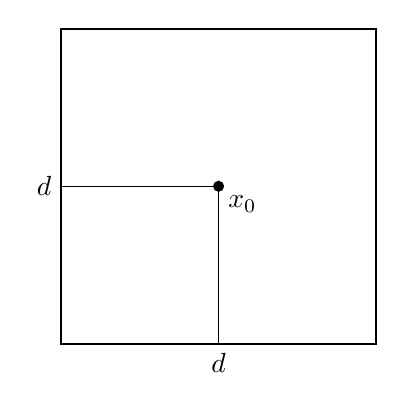
\begin{tikzpicture}[scale=2]
    % Рисуем квадрат
    \draw[thick] (0,0) rectangle (2,2);
    \draw[black, thin] (0,1)node[black, left] {$d$} -- (1, 1);
    \draw[black, thin] (1, 0) node[black, below] {$d$} -- (1, 1);

    % % \node[black, above] (0.5,1) {$d$};
    % \node[black] (1,0.5) {$d$};
    % Рисуем точку в центре
    \fill (1,1) node[black, below right] {$x_0$} circle (1pt); % размер точки можно изменить, подбирая значение радиуса
\end{tikzpicture}
$$
\end{minipage}


\subsection{Свойства множества меры нуль по Лебегу}
\begin{enumerate}
    \item В определении множества меры 0 можно использовать \textit{открытые} брусы
    
    \proof Пусть $\{I_i\}$ — открытые брусы  $M\subset \displaystyle\bigcup_iI_i$, то есть $M\subset\R^n$ — множество меры 0 по Лебегу
    
    Пусть $\{\bar I_i\}$ — замкнутые брусы $I_i$.
    \begin{equation*}
        \begin{aligned}
            M\subset\bigcup_iI_i \subset\bigcup_i\bar I_i, \, |I_i| = |\bar I_i|
        \end{aligned}
    \end{equation*}
    Если
    \begin{equation*}
        \forall\ve\, \exists\{I_i\}: M \subset \bigcup_iI_i: \sum_i|I_i|<\ve
    \end{equation*}
    то
    \begin{equation*}
        \forall\ve\, \exists\{\bar I_i\}: M \subset \bigcup_i\bar I_i: \sum_i|\bar I_i|<\ve
    \end{equation*}
    
    \textbf{Докажем в обратную сторону.} Пусть $\{I_i\}$ — набор замкнутых брусов
    \begin{equation*}
        I_i = [a^i_1, b^i_1]\times\ldots\times[a^i_n, b^i_n], \quad V_i = \sum_i|I_i|<\frac{\ve}{2^n}
    \end{equation*}
    Пусть 
    \begin{equation*}
        D_i = \left(\frac{a_1^i+b_1^i}{2} - (b_1^i-a_1^i) ; \frac{a_1^i + b_1^i}{2} + (b_1^i - a_1^i)\right) \times \ldots\times \left(\frac{a_n^i+b_n^i}{2} - (b_n^i-a_n^i) ; \frac{a_n^i + b_n^i}{2} + (b_n^i - a_n^i)\right)
    \end{equation*}
    $\implies V_2 = \displaystyle\sum_i|D_i| = 2^nV_1 < \ve$
    \qed

    \item $M$ — множество меры нуль, $L\subset M\Longrightarrow L$ — множество меры нуль
    
    \proof $L\subset M$ и $\forall\ve>0\exists$ не более чем счетное $\{I_i\}$:
    \begin{equation*}
        L\subset M\subset \bigcup_{i}I_i\text{ и }\sum|I+i|<\ve
    \end{equation*}
    по транзитивности это верно и для $L$\qed
    
    \item Не более чем счетное объединение множеств меры нуль — множество меры нуль
    
    \proof Пусть $\{M_k\}_{k=1}^{\infty}$ — счетное,\footnote[1]{Для конечного доказательство трививально} так как $\forall i\ M_k$ — множество меры нуль, то $\forall i,\forall \ve_i\ \exists$ не более чем счетное $\{I_i^k\}$: 
    \begin{equation*}
        M_k\subset I_i^k\text{ и }\sum|I_i^k|<\ve_k=\frac{\ve}{2^k}\forall \ve_k>0
    \end{equation*}

    Рассмотрим $M=\bigcup_{k=1}^{\infty} M_k$, тогда $M\subset \bigcup_{i,k} I_i^k$ и 
    \begin{equation*}
        \sum_{i,k}\underbrace{|I_i^k|}_{>0}<\sum_{k=1}^{\infty}\ve_k=\sum_{k=1}^{\infty}\frac{\ve}{2^k}=\ve\cdot\frac{1}{2}\cdot\frac{1}{\frac{1}{2}}=\ve
    \end{equation*}
    \qed

    \begin{itemize}
        \item \ex Пусть $\{M_i\}^N_{i=1}$ — конечный набор
        \begin{equation*}
            \begin{aligned}
                \varepsilon_1+\dots+\varepsilon_N&=\frac{N}{N+1}\varepsilon<\varepsilon\\
                \varepsilon_i&=\frac{\varepsilon}{N+1}
            \end{aligned}
        \end{equation*}
    \end{itemize}
 \end{enumerate}





\newpage
\section{Топология в $\mathbb{R}^n$}
\definition Пусть имеется $M\subset\mathbb{R}^n$. Точку $x_0\in M$ будем называть \textit{внутренней} точкой $M$, если $$\exists\ve>0:B_{\ve}(x_0)\subset M$$

\definition Точку $x_0\in M$ будем называть \textit{внешней} точкой $M$, если $$\exists\ve>0:B_{\ve}(x_0)\subset (\mathbb{R}^n\setminus M)$$

\ex $M=[0;1)$. тогда
\begin{equation*}
    \begin{cases}
        x=0.5&\text{ — внутренняя}\\
        x=0&\text{ — не внутренняя}\\
        x=2&\text{ — внешняя}
    \end{cases}
\end{equation*}

\definition Точку $x_0\in\mathbb{R}^n$ будем называть \textit{граничной} точкой $M$, если $$\forall \ve>0:\ \left(B_{\ve}(x_0)\cap M\right)\ne\varnothing\wedge B_{\ve}(x_0)\cap(\mathbb{R}^n\setminus M)\ne\varnothing$$ 

\mark $\partial M$ — множетсво всех граничных точек $M$

\ex $M=[0;1)\Longrightarrow x=0;1$ — граничные

\definition Точку $x_0\in M$ будем называть \textit{изолированной} точкой $M$, если $$\exists \ve>0:\ \stackrel{\circ}{B_{\ve}}(x_0)\cap M=\varnothing$$ 

\ex $M=[0;1]\cup \{3\}\Longrightarrow x=3$ — изолированная

\definition Точку $x_0\in\mathbb{R}^n$ будем называть \textit{предельной} точкой $M$, если $$\forall \ve>0:\ \stackrel{\circ}{B_{\ve}}(x_0)\cap M\ne\varnothing$$ 

\comment Из определения следует, что изолированные точки не являются предельными

\definition Точку $x_0\in\mathbb{R}^n$ будем называть \textit{точкой прикосновения} $M$, если $$\forall \ve>0:\ B_{\ve}(x_0)\cap M\ne\varnothing$$ 

\comment Точки прикосновения = изолированные точки $\oplus$ предельные точки

\definition Множество всех точек прикосновения $M$ называется \textit{замыканием} $M$ и обозначается как $\overline {M}$

\ex $M=(0;1)\cup(1;2]\Longrightarrow\overline{M}=[0;2]$

\ex $M=\{x\in[0;1]\colon x\in \mathbb{Q}\}\Longrightarrow\overline{M}=[0;1]$

\definition Множество $M\subset\mathbb{R}^n$ называется \textit{открытым}, если все его точки внутренние

\definition Множество $M\subset R^n$ называется замкнутым, если $\mathbb{R}^n\setminus M$ — открыто

\ex $\begin{cases}
    (0;1)&\text{ — открыто в $\mathbb{R}$}\\
    [0;1]&\text{ — замкнуто, т.к. $(-\infty;0)\cup(1;+\infty)$ открыто в $\mathbb{R}$}\\
    [0;1)&\text{ — ни открыто, ни замкнуто в $\mathbb{R}$}
\end{cases}$

\definition Множество $K\subset\R^n$ называется \textit{компактом}, если из $\forall$ его покрытия открытыми множествами можно выделить конечное подпокрытие

\comment Если хотя бы для какого-то покрытия это не выполняется, то $K$ — не компакт

\ex Пусть $M=(0,1)$ покроем $\left\{A_n=\left(0;1-\frac{1}{n}\right)\right\}_{n=1}^\infty$

При $n\rightarrow\infty$ $M\subset \displaystyle\bigcup_{n=1}^\infty A_n$, но $\forall$ фиксированного $N$: $M\not\subset\displaystyle\bigcup_{n=1}^{\infty}\Longrightarrow$ не компакт

\definition Множество $M\subset \mathbb{R}^n$ — называется \textit{ограниченным}, если $$\exists x_0\in\mathbb{R}^n\text{ и }\exists r>0\text{, такой что }M\subset B_{r}(x_0)$$

\subsection{Критерий замкнутости}
% Наличие социофобии

\theorem $M$ — замкнуто $\Longleftrightarrow$ $M$ содержит \textbf{все} cвои предельные точки

\proof Докажем необходимость и достаточность
\begin{enumerate}
    \item \textit{(Необходимость)} Докажем $\Longrightarrow$ от противного
    \begin{itemize}
        \item Пусть $x_0$ — предельная для $M$ и $x_0\notin M$. Тогда, $\forall\ve>0\ \stackrel{\circ}{B_{\ve}}(x_0)\cap M\ne\varnothing\text{ и }x_0\in\mathbb{R}^n$
        \item По условию $M$ — замкнуто, то есть $\mathbb{R}^n\setminus M$ — открыто $\Longrightarrow$ все его точки внутренние и $\exists r>0$:
        $$B_{r}(x_0)\subset\mathbb{R}^n\setminus M\Longrightarrow\stackrel{\circ}{B_r(x_0)}\subset\mathbb{R}^n\setminus M\text{ и }\stackrel{\circ}{B_r}(x_0)\cap M=\varnothing$$

        Пришли к противоречию $\Longrightarrow$ $M$ содержит все свои предельные точки\qed
    \end{itemize}
    \item \textit{(Достаточность)} Докажем $\Longleftarrow$
    
    Пусть $y_0$ — не является предельной для $M$, то есть $y_0\in\mathbb{R}^n\setminus M\Longrightarrow\exists r>0$:
    \begin{equation*}
        \begin{cases}
            \stackrel{\circ}{B_{r}}(y_0)\cap M=\varnothing\\
            y_0\in\mathbb{R}^n\setminus M
        \end{cases}\Longrightarrow B_r(y_0)\subset \mathbb{R}^n\setminus M
    \end{equation*}
    $\Longrightarrow\mathbb{R}^n\setminus M$ — открытое и состоит из всех точек, не являющихся предельными $\Longrightarrow$ $M$ — замкнуто по определению\qed
\end{enumerate}

\newpage
\section{Компакты в $\mathbb{R}^n$}
\subsection{Замкнутый брус — компакт}
\theorem Пусть $I\subset\mathbb{R}^n$ — замкнутый брус $\Longrightarrow I$ — компакт

\proof Пойдем от противного

Пусть $I=[a_1;b_1]\times\ldots\times[a_n;b_n]$
\begin{enumerate}
    \item Положим, что $I$ — не компакт. Значит, существует его покрытие $\{A_{\alpha}\}$ — открытые множества, такие что $I\subset \{A_{\alpha}\}$, не допускающее выделения конечного подкпорытия
    \item Поделим каждую сторону пополам. Тогда, $\exists I_1$, такой что не допускает конечного подпокрытия. Иначе, $I$ — компакт
    \item Аналогично, повторим процесс и получим систему вложенных брусов: $$I\supset I_1\supset I_2\supset \ldots$$
    То есть на каждой стороне возникает последовательность вложенных отрезков, которые стягиваются в точку $a=(a_1,\ldots,a_n)$
    
    При этом, $a\in I_i\ \forall i\text{ или } a\in\displaystyle\bigcap_{i=1}^{\infty}I_i$

    \item $a\in I\Longrightarrow a\in \bigcup A_{\alpha}\Longrightarrow\exists \alpha_0:a\in \underbrace{A_{\alpha_0}}_{\text{открытое}}\Longrightarrow\exists \ve>0: B_{\ve}(a)\subset A_{\alpha_0}$

    \item Мы знаем, что $d(I_i)\mapsto0$ при $i\mapsto\infty$. Тогда, $$\exists N:\forall i > N\ I_i\subset B_{\ve}(a)\subset A_{\alpha_0}$$
    Получается, что $\forall i>N\ I_i$ покрывается одним лишь $A_{\alpha_0}$ из системы $\{A_{\alpha}\}$

    Получаем противоречие тому, что любое $I_i$ не допускает конечного подпокрытия, а у нас получилось, что $I_i\in A_{\alpha_0}\forall i>N$
\end{enumerate}

\comment Любое ограниченное множество можно вписать в замкнутый брус. Потому что можно вокруг него описать шарик, который точно можно вписать в брус

\subsection{Критерий компактности}
\theorem $K\subset \mathbb{R}^n$. $K$ — компакт $\Longleftrightarrow$ $K$ замкнуто и ограниченно

\proof Докажем необходимость $(\Longrightarrow)$
\begin{itemize}
    \item \textit{Ограниченность.} $K$ — компакт, значит монжо выбрать покрытие $\{B_{m}(0)\}_{m=1}^{\infty}$ — открытые шары
    
    Тогда, $\exists m_0:K\subset \displaystyle\bigcup_{m=1}^{m_0} B_m(0)\Longrightarrow K\subset B_{m_0}(0)\Longrightarrow$ по определению $K$ — ограничено

    \item \textit{Замкнутость.} Пойдем от противного. $K$ — компакт, тогда возьмем $\{B_{\frac{\delta(x)}{2}}(0)\}_{x\in K}$ — покрытие открытыми шарами, где $\delta(x)=\rho(x,x_0)$. $x_0$ — предельная точка, которая $\notin K$ (или же $\in \mathbb{R}^n\setminus K$)
    
    Так как $K$ — компакт, $\exists x_1,\ldots, x_s:K\subset\displaystyle\bigcup_{i=1}^{s} B_{\frac{\delta(x_i)}{2}}(x_i)$

    Пусть $\delta=\min\limits_{1\leqslant i\leqslant s}{\delta(x_i)}$, тогда
    \begin{equation*}
        \begin{aligned}
            B_{\frac{\delta}{2}}(x_0)\cap\bigcup_{i=1}^{s}B_{\frac{\delta(x_i)}{2}}(x_i)=\varnothing&\Longrightarrow B_{\frac{\delta}{2}}(x_0)\subset\mathbb{R}^n\setminus K\\
            &\Longrightarrow\stackrel{\circ}{B}_{\frac{\delta}{2}}(x_0)\cap K=\varnothing
        \end{aligned}
    \end{equation*}

    Значит, $x_0$ \textit{не является предельной точкой} $K$, что противоречит нашему предположению
\end{itemize}

\proof Докажем достаточность

$K$ — замкнуто и ограничено $\Longrightarrow r>0:B_r(0)\supset K\Longrightarrow\exists I$ — замкнутый брус, такой что 
$$K\subset I\text{ и }I=[-r;r]^n\supset K$$
% тут позже будет картинка

Пусть $A_{\alpha}$ — произвольное покрытие открытыми множествами для $K$. Тогда, $I\subset \{A_{\alpha}\}\cup\underbrace{\{\mathbb{R}^n\setminus K\}}_{\text{открыто}}$. Так как $I$ — компакт, то $\exists $ конечное подпокрытие 
$$\{A_{\alpha_i}\}_{i=1}^m\cup\{\mathbb{R}^n\setminus K\}\supset I\supset K\text{ — покрытие для $I$}$$

Значит, $K\subset\{A_{\alpha_i}\}_{i=1}^{m}$ — конечное и $\{A_{\alpha}\}$ — произвольное, тогда $K$ — компакт по определению\qed

\newpage
\section{Теорема Вейерштрасса о непрерывной функции на компакте. Колебания функции}

\subsection{Теорема Вейерштрасса о непрерывной функции на компакте}
\theorem Пусть $K\in \R^n$ — компакт и функция $f: K\mapsto \R$ - непрерывная. Тогда $f$ на $K$ достигает наибольшее и наименьшее значения.

\proof 
\begin{itemize}
    \item \textit{Ограниченность.} От противного: пусть существует последовательность $\{x^k\} \subset K \,:\, |f(x^k)| > k$. Из ограниченности $K$ следует ограниченность последовательности $\{x^k\}$, и как следствие ограничены последовательности отдельных коордиант:
    \begin{equation*}
        |x_i^k| = \sqrt{\sum_{i=1}^n|x_i^k|} = ||x^k|| \le C \quad \text{для некоторого }C
    \end{equation*}

    По теореме Больцано-Вейерштрасса у $\{x_1^k\}$ существует сходящаяся подпоследовательность $x_1^{k_{j_1}} \to a_1, j_1 \to \infty$. Для последовательности $\{x_2^{k_{j_1}}\}$ существует сходящаяся последовательность $x_2^{k_{j_2}} \to a_2, j_2 \to \infty$. И т.д. Получаем сходящуюся подпоследовательность:
    \begin{equation*}
        x^{k_j} = (x_1^{k_j}, x_2^{k_J}, \ldots, x_n^{k_j})\to(a_1, a_2, \ldots, a_n) = a
    \end{equation*}

    Точка $a$ — предельная для $K$. В силу замкнутости $K$ т. $a\in K$. А из непрерывности функции $f$ получаем $f(x^{k_j}) \to f(a)$. А с другой стороны, $f(x^{k_j})\to\infty$ из выбора исходной последовательности. \textbf{противоречие}

    \item \textit{Достижение наибольшего (наименьшего) значения.} Итак, мы доказали, что $f$ — ограничена на $K$. Выберем последовательность $\{x^k\}$:
    \begin{equation*}
        \sup_K f - \frac{1}{k_j} \le f(x^{k_j}) \le \sup_K f
    \end{equation*}
    в силу непрерывности $f$:
    \begin{equation*}
        \sup_K f \le f(a) \le \sup_K f
    \end{equation*}
    Получаем $f(a) = \displaystyle\sup_K f$, т.е. максимальное значение достиигается в точке $x = a$. Для $\displaystyle\inf_K f$ доказательство аналогично
    \qed
\end{itemize}
\subsection{Расстояние между двумя множествами}
\definition Расстоянием между двумя множествами $X$ и $Y$, где $X, Y \subset \R^n$ будем называть число $\rho(X, Y)$:
\begin{equation*}
    \rho(X, Y) = \inf_{\substack{x\in X\\y\in{Y}}} ||x-y||
\end{equation*}

\textbf{Примеры:}\\
\begin{enumerate}
    \item $X\cap Y \ne \varnothing \implies \rho(X, Y) = 0$
    \item $\rho(X, Y) =0 \implies X \cap Y \ne \varnothing?$ --- нет, пример: $X = (0, 1); (Y = (1; 2)$ - не компакты
\end{enumerate}

\subsection{Расстояние между непересекающимися компактами}
\theorem Если $K_1, K_2 \subset \R^n$ — компакты и $K_1 \cap K_2 = \varnothing$, то $\rho(K_1, K_2)$ > 0

\proof Функция $f(x,y)=||x-y||$ определена на $K_1\times K_2 \subset \R^n\times\R^n = \R^{2n}$, причем $f$–непрерывная функция.

По теореме Вейерштрасса эта функция достигает своего максимального и минимального значений. Т.е. существуют $x_0 \in K_1, y_0 \in K_1: f(x_0, y_0) = \rho(K_1, K_2)$. А $f(x_0,y_0) = 0$ тогда и только тогда, когда $x_0 = y_0$. \qed

\subsection{Колебание функции на множестве}
\definition Колебанием функции $f$ на множестве $M\subset \R^n$ будем называть число $\omega(f, M)$:
\begin{equation*}
    \omega(f, M) = \sup_{x, y\in M}|f(x) - f(y)| = \sup_{x\in M} - \inf_{y\in M} f(y)
\end{equation*}

\subsection{Колебание функции в точке}
\definition Колебанием функции $f$ в точке $x_0 \in M \subset\R^n$ будем называть число
\begin{equation*}
    \omega(f, x_0):= \lim_{r \to 0+} \omega(f, B_r^M(x_0)), \quad \text{где } B_r^M = B_r(x_0)\cap M
\end{equation*}

\textbf{Напоминание:} По определению, функция $f: M\to \R$ непрерывна в точке $x_o\in M$, если $\forall \ve > 0\,\, \exists\delta > 0: \forall x\in M \quad |x-x_0| < \delta\,\, \iff x\in B_{\delta}(x_0) \cap M$ верно $|f(x) - f(x_0)| < \ve$

\subsection{Колебание функции, непрерывной в точке}
\theorem Пусть $x_0 \in M \subset \R^n; \,\, f: M\mapsto\R$. $f$ — непрерывна в точке $x_0 \iff \omega(f, x_0) = 0$

\proof
\begin{itemize}
    \item \textit{Необходимость}\\
        
        $f$ — непрерывна в т. $x_0 \in M \implies \forall \ve > 0 \,\, \exists\delta > 0:\,\, \forall x \in B_{\delta}(x_0)\cap M = B_{\delta}^M(x_0) \implies |f(x) - f(x_0)| < \frac{\ve}{3}$\\
        Рассмотрим $\omega(f, x_0) := \displaystyle\lim_{\delta\to0+} \omega(f, B_{\delta}^M(x_0))$:
        \begin{equation*}
            \begin{aligned}
                \omega(f, B_{\delta}^M(x_0)) = \sup_{x, y \in B_{\delta}(x_0)}|f(x) - f(y)| \le \sup_{x\in B_{\delta}(x_0)} |f(x) - f(x_0)| + \sup_{y\in B_{\delta}(x_0)} |f(y) - f(x_0)| \le \frac{2\ve}{3} < \ve
            \end{aligned}
        \end{equation*}
        При $\ve\to0 \implies \delta\to0$ и $\omega(f, B_{\delta}^M(x_0))\to0$, т.е. $\omega(f, x_0) = 0$

    \item \textit{Достаточность}

        Пусть $0 = \omega(f, x_0) := \displaystyle\lim_{\delta\to0+} \omega(f, B_{\delta}^M(x_0))$, т.е.
        \begin{equation*}
            \forall \ve > 0 \,\, \exists\delta > 0: \quad \forall x, y \in B_{\delta}^M(x_0) \quad \sup_{x, y\in B_{\delta}^M(x_0)} |f(x)-f(y)| < \ve
        \end{equation*}
        Получаем, что
        \begin{equation*}
            \forall \ve > 0 \,\, \exists \delta > 0: \forall x \in B_{\delta}^M(x_0) \implies |f(x)-f(x_0)| < \ve \implies
        \end{equation*}
\end{itemize}\qed


\definition Если какое-то свойство не выполняется лишь на множестве меры нуль, то говорят, что это свойство выполняется почти всюду.

\textbf{Пример:} $f(x) = \begin{cases}
        1, x \in \R\backslash \mathbb{Z}\\
        0, x \in \mathbb{Z}
    \end{cases}$ --- непрерывна почти всюду на $\R$

\subsection{Пересечение разбиений бруса}
\definition Пусть $\T_1 = \{I^1_k\}$ и $\T_2 = \{I^2_m\}$ — два разбиения бруса $I \subset \R^n$. 

Пересечением разбиений $(\T_1 \cap \T_2)$ будем называть мн-во всех брусов $\{I_{ij}\}: \forall I_{ij}$
$\begin{cases}
    1) \exists k: I_{ij} \in \{I^1_k\}\\
    2) \exists m: I_{ij} \in \{I^2_m\}\\
    3) \{I_{ij}\} - \text{ разбиение бруса } I   
\end{cases}$

\subsection{Критерий Лебега об интегрируемости функции по Риману}
\theorem Если $I\subset \R^n$ — замкнутый невырожденный брус, $f: I\to\R$, то $f\in R(I) \iff f$ ограничена и непрерывна почти всюду на $I$

\proof 
\begin{itemize}
    \item \textit{Необходимость}
    
     Если $f$ интегрируема, то она ограничена по необходимому условию интегрируемости. Осталось показать, что множества разрыва меры нуль. От противного: пусть это не так.

    Обозначим множество всех точек разрыва ф-ии $f$ на $I$ за $T$ и заметим, что $T = \displaystyle\bigcup_{k\in\mathbb{N}}T_k$, где\\
    $T_k = \{x\in I | \omega(f, x) \ge \frac{1}{k}\}$. Если $T$ не меры нуль, то существует $T_{k_0}$ не меры нуль (если они все меры нуль, то по свойству множеств меры нуль счетное объединение таких множеств тоже было бы меры нуль).

    Для произвольного разбиения $\T = \{I_i\}_{i=1}^m$ бруска $I$ разобъем эти бруски на две кучи: первая $A = \{I_i | I_i\cap T_{k_0} \ne \varnothing, \omega(f, I_i) \ge \frac{1}{2k_0}\}$ и вторая $B = \T\backslash A$. Покажем что $A$ является покрытием множества $T_{k_0}$, т.е. $T_{k_0} \subset \displaystyle\bigcup_{i: I_i\in A} I_i$ любая точка $x\in T_{k_0}$ является либо
    \begin{itemize}
        \item[a)] внутренней для некоторого бруска $I_i$. В этом случае $\omega(f, I_i) \ge \omega(f, x) \ge \frac{1}{k_0} > \frac{1}{2k_0}$, т.е. $I_i \in A$, либо
        \item[b)] точка $x$ лежит на границе некоторого количества брусков (не более чем $2^n$ штук). Тогда хотя бы на одном из них колебание $\omega(f, I_i) \ge \frac{1}{2k_0}$ (т.е. $I_i \in A$): если бы такого не нашлось, то в любой малой окрестности $B_{\ve}(x)$ выполняется следующее:
        \begin{equation*}
            \omega(f, x) \le \sup_{x', x''\in B_{\ve}(x)} |f(x')-f(x'')| \le \sup_{x'\in B_{\ve}(x)}|f(x')-f(x)| + \sup_{x''\in B_{\ve}(x)}|f(x)-f(x'')| < \frac{1}{2k_0} + \frac{1}{2k_0} = \frac{1}{k_0}
        \end{equation*}
        т.е. $x\not\in T_{k_0}$ --- \textbf{противоречие}.
    \end{itemize}

    Таким образом, каждая точка $x\in T_{k_0}$ покрывается некоторым бруском $I_i \in A$, т.е. $A$ - покрытие $T_{k_0}$. Тогда существует $c: \displaystyle\sum_{i:I_i\in A}|I_i| \ge c > 0$ для всех разбиений $\T$ (если бы меняя разбиения мы могли получить сумму объемов этих брусков сколь угодно маленькую, то получилось бы, что $T_{k_0}$ меры нуль)

    Возьмем два набора отмеченных точек $\xi^1$ и $\xi^2$. На брусках из кучки $B$ будем их брать одинаковыми, т.е. для $I_i\in B \,\, \xi_i^1 = \xi_i^2$. А на брусках из кучки $A$ будем брать такие, чтобы 
    \begin{equation*}
        f(\xi_i^1) - f(\xi_i)^2 \ge \frac{1}{3k_0} \text{ (у нас там колебания} \ge 1/2k_0, \text{ так что такие найдутся)}
    \end{equation*}

    Получаем:
    \begin{equation*}
        \begin{aligned}
            |\sigma(f, \T, \xi^1) - \sigma(f, \T, \xi^2) 
            = \left|\sum_i(f(\xi_i^1) - f(\xi_i^2))|I_i|\right|\\
            = \left|\sum_{i: I_i\in A}(f(\xi_i^1) - f(\xi_i^2))|I_i| + \sum_{i:I_i\in B}(f(\xi_i^1) - f(\xi_i^2))|I_i|\right|\\
            = \left|\sum_{i: I_i\in A} (f(\xi_i^1) - f(\xi_i^2))|I_i|\right| \ge \frac{1}{3k_0} \sum_{i:I_i\in A}|I_i| \ge \frac{c}{3k_0} > 0
        \end{aligned}
    \end{equation*}
    т.е. интегральные суммы не могут стремиться к одному и тому же числу, значит $f$ не интегрируема --- \textbf{противоречие}.

    \item \textit{Достаточность}

    Для любого $\ve > 0$ рассмотрим $T_{\ve} = \{x\in I| \omega(f, x) \ge \ve\}$. Покажем, что это множество - компакт. Ограниченность очевидна (подмножества бруска), а замкнутость проверим от противного. Пусть $a$ - предельная точка $T_{\ve}: \,\, a\not\in T_{\ve}$. Т.к. она предельная, то существует $\{x^k\}: x^k \in B_{\frac{1}{k}}(a)$. Т.к. $B_{\frac{1}{k}}$ - открытые шары, то наши точки лежат в них с окрестностями, т.е. сущесвтуют $\delta_k : B_{\delta_k}(x_K) \subset B_{\frac{1}{k}}(a)$. Тогда
    \begin{equation*}
        \omega(f, B_{\frac{1}{k}}(a)) \ge \omega(f, B_{\delta_k}(x_K)) \ge \omega(f, x_k) \ge \ve
    \end{equation*}
    Переходя к пределу $k\to\infty : \omega(f, a) \ge \ve$, т.е. $a\in T_{\ve}$ - противоречие. Значит $T_{\ve}$ - замкнуто, и, следовательно, компактно.

    Множество $T_{\ve}$ - множество меры нуль (как подмножество множества меры нуль). Значит, его можно покрыть не более чем счетным объединением открытых брусков $I_i: \displaystyle\sum_i|I_i| < \ve$. Т.к. это открытое покрытие, а $T_{\ve}$ - компакт, то существует конечное подпокрытие: $T_{\ve} \subset \displaystyle\bigcup_{i=1}^m I_i$, при этом $\displaystyle\sum_{i=1}^m |I_i| < \ve$.

    Обозначим три множества: $C_1 = \displaystyle\bigcup_{i=1}^mI_i, \quad C_2 = \displaystyle\bigcup_{i=1}^mI_i', C_3 = \displaystyle\bigcup_{i=1}^mI_i''$, где $I_i', I_i''$ - бруски, полученные гомотетией с центром в центре $I_i$ с коэффициентом 2 и 3 соответственно.

    Заметим, что
    \begin{itemize}
        \item[a)] $|C_3| \le \displaystyle\sum_{i=1}^m|I_i''|| = 3^n \displaystyle\sum_{i=1}^m|I_i| < 3^n \ve$
        \item[b)] расстояние $\rho(\partial C_2, \partial C_3) = \delta_1 > 0$ (теорема про расстояние между компактами)
        \item[c)] Множество $K = I\backslash(C_2\backslash \partial C_2)$ - компакт. Кстати, любое множество с диаметром меньше $\delta_1$ либо польностью лежит в $C_3$, либо полностью в $K$.
        \item[d)] $T_{\ve} \cap K = \varnothing$, т.к. $T_{\ve} \subset C_1 \subset C_2$. Следовательно, $\forall x\in K \,\, \omega(f, x) < \ve$. Тогда по теореме Кантора-Гейне $\exists \delta_2 > 0: \,\, \forall x\in K \,\, \omega(f, B_{\delta_2}(x)) < \ve + \ve = 2\ve$
    \end{itemize}

    Выберем $\delta = \min\{\delta_1, \delta_2\}$. Тогда для любых разбиений $\T_1 = \{I_k^1\}, \T_2 = \{I_i^2\}: \lambda{\T_1} < \delta, \lambda(\T_2) < \delta$

    Рассмотрим пересечение этих разбиений $\T = \T_1 \cap \T_2$, т.е. такое разбиение $\T = \{I_{ik}\}$, что $I_k^1 = I_{i_1k} \bigsqcup\ldots\bigsqcup I_{i_mk}$ и $I_i^2 = I_{ik_1} \bigsqcup \ldots\bigsqcup I_{ik_l}$. Очевидно $\lambda(\T) < \delta$.

    Для произвольных наборов отмеченных точек:
    \begin{equation*}
        |\sigma(f, \T_1, \xi^1) - \sigma(f, \T_2, \xi^2)| \le |\sigma(f, \T_1, \xi^1) - \sigma(f, \T, \xi)| + |\sigma(f, \T_2, \xi^2) - \sigma(f, \T, \xi)|
    \end{equation*}

    Рассмотрим отдельное слагаемое:
    \begin{equation*}
        \begin{aligned}
            |\sigma(f, \T_1, \xi^1) - \sigma(f, \T, \xi)| = \left|\sum_{i, j}(f(\xi_i^1) - f(\xi_{ij}))|I_{ij}\right|\
            \le \sum_{I_{ij}\in C_3}|f(\xi_i^1) - f(\xi_{ij})||I_{ij}| + \sum_{I_{ij\in K}}|f(\xi_i^1)-f(\xi_{ij})||I_{ij}|\le 2M\cdot e^n\ve + 2\ve |I| = \epsilon(2M\cdot 3^n + 2|I|)
        \end{aligned}
    \end{equation*}
    т.к. $f$ ограничена некоторой константой $M$ и см пункты $a), d)$, то

    Т.к. для $(\T_2, \xi^2)$ все выкладки аналогичные, то получаем:
    
    \begin{equation*}
         |\sigma(f, \T_1, \xi^1) - \sigma(f, \T, \xi)| \le \epsilon(2M\cdot 3^n + 2|I|)
    \end{equation*}

        Следовательно, существует предел $\displaystyle\lim_{\lambda(\T)\to0}\sigma(f, \T, \xi)$ (Критерий коши для функций)
\end{itemize} \qed

\subsection{Измельчение разбиения}
\definition Разбиение $\T_1 = \{I^1_k\}$ будем называть измельчением разбиения $\T_2 = \{I^2_m\}$, если $\forall k \,\, \exists m: I_k^1 \in I_m^2 \implies \T = \T_1\cap \T_2$ является измельчением $\T_1$ и $\T_2$



\newpage
\section{Суммы Дарбу}
\subsection{Нижняя и верхняя суммы Дарбу}
\definition Пусть $I$ - замкнутый брус, $f: I\mapsto \R$, $\T = \{I_i\}_{i=1}^{K}$ -разбиение бруса $I$, $m_i = \displaystyle\inf_{I_i} (f)$, и $M_i = \displaystyle\sup_{I_i} (f)$. Тогда числа $\underline{S}(f, \T) = \sum_{i=1}^{K}m_i|I_i|$ и $\overline{S}(f, \T) = \sum_{i=1}^KM_i|I_i|$ будем называть \textbf{нижней и верхней суммой Дарбу} соответственно

\subsection{Нижняя сумма Дарбу не больше верхней}
\theorem \begin{equation*}
    \us(f, \T) = \int_{\xi}\sigma(f, \T, \xi) \le \sup_{\xi}\sigma(f, \T, \xi) = \os(f, \T)
\end{equation*}

\proof
\begin{equation*}
    \begin{aligned}
    &\us(f, \T) = \sum_{i=1}^{K}m_i|I_i| = \sum_{i}\inf_{\xi_i}(f(\xi_i))|I_i| = \inf_{\xi}\sum_{i}f(\xi_i)|I_i| = \inf_{\xi}\sigma(f, \T, \xi) \le\\
    &\sup_{\xi}\sigma(f, \T, \xi) = \sum_i (f(\xi_i))|I_i| = \sum_{i}M_i|I_i| = \os(f, \T)
    \end{aligned}
    \end{equation*}

\subsection{Монотонность сумм относительно измельчений разбиения}
\theorem Пусть $\tilde{\T}$ — измельчение разбиения $\T$, тогда
\begin{equation*}
    \us(f, \T) \le \us(f, \tilde{\T}) \le \os(f, \tilde{\T}) \le \os(f, \T)
\end{equation*}\qed

\proof Если $L \subset M$, то $\inf L \ge \inf M$ и $\sup L \le \sup M$, тогда:
\begin{equation*}
    \us(f, \T) \le \us(f, \tilde{\T}) \underset{\text{по 6.2}}{\le} \os (f, \tilde{\T}) \le \os (f, \T)
\end{equation*}\qed

\subsection{Никакая нижняя сумма Дарбу не больше какой-либо верхней суммы на том же брусе}
\theorem $\forall \T_1, \T_2 : \quad \us(f, \T_1) \le \os(f, \T_2)$

\proof $\forall \T_1, \T_2$ рассмотрим $\tilde{\T} = \T_1 \cap \T_2$, тогда по 6.3:
\begin{equation*}
    \us(f, \T_1) \le \us(f, \tilde{\T}) \le \os(f, \tilde{\T}) \le \os(f, \T_2)
\end{equation*} \qed

\subsection{Верхние и нижние интегралы Дарбу}
\definition \textbf{Верхним и нижним интегралом} Дарбу будем называть числа 
\begin{equation*}
    \oi := \inf_{\T}\os(f, \T) \qquad \ui := \sup_{\T}\us(f, \T)
\end{equation*}
соответственно


\subsection{Интеграл Дарбу как предел сумм Дарбу}
\theorem Пусть $I\subset \R^n$ — замкнутый брус, а $f: I \mapsto \R$ — ограничена. Тогда:
\begin{equation*}
    \oi = \lim_{\Delta_{\T}\to0}\os(f, \T) \qquad \text{и} \qquad \ui = \lim_{\Delta_{\T} \to 0} \us(f, \T)
\end{equation*}

\proof Докажем, что $\ui = \displaystyle\lim_{\Delta_{\T} \to 0} \us(f, \T) \quad (= \displaystyle\sup_{\T} \us (f, \T))$
\begin{enumerate}
    \item $f$-ограничена на $I$, то $\exists C > 0: \forall x \in I\quad |f(x)|< C$
    \item т.к. по определению $\underline{I} = \displaystyle\sup_{\T}\us(f, \T)$, то $\forall \ve > 0 \,\, \exists\T_1 = \{I_i^1\}_{i=1}^{m_1}:\ \ui-\ve < \us(f, \T_1) \le \ui < \ui + \ve$
    \item Пусть $G = \displaystyle\bigcup_{i=1}^{m_1}\partial I_i^1$ - объединение границ брусов (без повторов). Тогда $G$ множество меры нуль по Лебегу (т.к. границы --- мн-ва меры нуль по Лебегу)
    \item Пусть $\T_2$ - произвольное разбиение $I: \,\, \T_2 = \{I_i^2\}_{i=1}^{m_2}$ \\
    Рассмотрим две кучки брусов:\\
    \begin{equation*}
    \begin{aligned}
        A = \{I_i^2 \in \T_2: I_i^2 \cap G \ne \varnothing\} \qquad \text{и} \qquad B = \T_2\backslash A \implies\\
        \forall \ve > 0 \,\, \exists \delta > 0 : \forall \T_2: \Delta_{\T_2} < \delta \text{ верно, что } \sum_{I_i^2 \in A} |I_i^2| < \epsilon
    \end{aligned}
    \end{equation*}
    по определению множества меры нуль, а также т.к. $A$ - покрытие замкнутыми брусами, а $G$ - мн-во меры нуль.

    \item С другой стороны $\forall I_i^2 \in B$ верно, что $I_i^2 \in \T_1 \cap \T_2$
\end{enumerate}

Хотим рассмотреть 
\begin{equation*}
\begin{aligned}
    |\ui - \us(f, \T_2)| = |I-\us(f, \T_1\cap \T_2) + \us(f, \T_1\cap \T_2) -\us(f, \T_2)| &\le \underbrace{|I-\us(f, \T_1\cap \T_2)|}_* + \underbrace{|\us(f, \T_1\cap \T_2) -\us(f, \T_2)|}_{**} \\
    &< \ve + 2M\ve = \ve(1+2M)
\end{aligned}
\end{equation*}

\begin{itemize}
    \item[*] из п.2: $\ui - \ve < \us(f, \T_1) \le \us(f, \T_1\cap \T_2) \le \ui < \ui + \ve \implies |\ui - \us(f, \T_1\cap\T_2)| < \ve$\\
    \item[**] \begin{equation*}
        \begin{aligned}
            \left|\us(f, \T_1\cap\T_2) - \us(f, \T_2)\right| &= \left|\sum_{I_i^2\in B}m_i|I_i^2| + \sum_{I_i^2\in \T_2\cap A}m_i|I_i^2| - \sum_{I_i^2\in B}m_i|I_i^2| - \sum_{I_i^2\in A}m_i|I_i^2|\right|\\
            % &\le \sum_{I_i^2\in \T_2\cap A}m_i|I_i^2| - \sum_{I_i^2\in A}m_i|I_i^2||\\
            &\le \left|\sum_{I_i^2\in \T_2\cap A}m_i|I_i^2|\right| + \left|\sum_{I_i^2\in A}m_i|I_i^2|\right|\\
            &\le 2\left|\sum_{I_i^2\in A}m_i|I_i^2|\right|\\
            &< 2M\left|\sum_{I_i^2\in A}|I_i^2|\right|\\
            &\le 2M\ve
        \end{aligned}
    \end{equation*}
\end{itemize}\qed


\newpage
\section{Критерий Дарбу. Теорема Фубини}
\subsection{Критерий Дарбу интегрируемости функции по Риману}
$I\in\mathbb{R}^n\text{ — замкнутый брус, } f:I\mapsto \mathbb{R}, f\in \mathcal{R}(I)\Longleftrightarrow f$ — ограничена на $I$ и $\ui=\oi$

\proof Необходимость 
\begin{itemize}
    \item $f\in\riman{I}\Longrightarrow$ по необходимому условию интегрируемости функции по Риману на замкнутом брусе, $f$ — ограничена на $I$
    \item Покажем, что $\underline{\mathcal{I}}=\mathcal{I},\overline{\mathcal{I}}=\mathcal{I}\Longrightarrow\underline{\mathcal{I}}=\overline{\mathcal{I}}$
    
    \begin{enumerate}
        \item $f\in\riman{I}\Longrightarrow\forall \ve >0\ \exists \delta >0\ \forall(\mathbb{T},\xi):\Delta_{\mathbb{T}}<\delta\hookrightarrow|\sigma(f,\mathbb{T},\xi)-\mathcal{I}|<\ve$
        \item $\ui=\sup\limits_{\mathbb{T}}=\lim\limits_{\Delta\rightarrow 0}=\us(f,\mathbb{T})\Longrightarrow |\ui-\us|<\ve$
        
        $\forall \ve>0\ \exists\delta\ \exists\mathbb{T}:\Delta_{\mathbb{T}}<\delta: |\ui-\us|<\ve$
        \item $\us(\mathbb{T},\xi)=\inf\limits_{\xi}\sigma(f,\mathbb{T},\xi)$
        
        $\forall\mathbb{T},\ \forall \ve>0\ \exists \xi:|\us-\sigma|<\ve$
    \end{enumerate}
\end{itemize}

$|\mathcal{I}-\ui|\leqslant|\mathcal{I}-{\ui}-\sigma+\sigma+{\us}-\us|\leqslant|\mathcal{I}-\sigma|+|\ui-\us|+|\sigma-\us|<3\ve$\qed

\proof Достаточность

$f$ — ограничена и $\ui=\oi$. Имеем 
\begin{equation*}
    \us(f,\mathcal{T})=\inf\limits_{\xi}\leqslant\sigma(f,\mathbb{T},\xi)\leqslant \sup\limits_{\xi}(f,\mathbb{T},\xi)=\os(f,\mathbb{T})
\end{equation*}

Тогда, при $\lim\limits_{\Delta\rightarrow 0} \us=\ui,\ \lim\limits_{\Delta\rightarrow0}\os=\oi$ получаем $\ui=\oi$\qed


\subsection{Интегрирование по допустимым множествам}

\definition Множество $D\subset\mathbb{R}^n$ называется \textit{допустимым}, если

\begin{itemize}
    \item $D$ — ограниченно
    \item $\partial D$ — множество меры нуль по Лебегу
\end{itemize}

\definition Пусть $D\subset\mathbb{R}^n, f:D\rightarrow\mathbb{R}$. Тогда, интегралом Римана $f$ по $D$ называется число $\mathcal{I}$:
\begin{equation*}
    \mathcal{I}=\int\limits_{D}f(\overline{x})\d{\overline{x}}=\int\limits_{I\supset D}f\cdot \chi_{D}(\overline{x})\d{\overline{x}}\text{, где }\chi_{D}=\begin{cases}
        1,\overline{x}\in D\\
        0,\overline{x}\in D
    \end{cases}
\end{equation*}

% \begin{equation*}
%     \chi_{D}=\begin{cases}
%         1,\overline{x}\in D\\
%         0,\overline{x}\in D
%     \end{cases}
% \end{equation*}

\textbf{Корректность определения.} Пусть $I_1\supset D, I_2\supset D$, тогда 
\begin{equation*}
    \int\limits_{I_1} f\cdot\chi_D\d{x}\text{ и }\int\limits_{I_2}f\cdot\chi_{D}\d{x}
\end{equation*}

либо существуют и равны, либо оба не существуют вообще

Покажем существование
\begin{itemize}
    \item $f\cdot\chi_D\in\riman{I_1}\Longrightarrow$ по критерию Лебега $f\cdot\chi_D$ ограничена на $I_1\Longrightarrow$ $f\cdot\chi_D$ ограничена на $D\Longrightarrow f$ ограничена на $D\Longrightarrow f\cdot\chi_D$ ограничена на $I_2$
    \item $f\cdot\chi_D\in\riman{I_1}\Longrightarrow$ по критерию Лебега $f\cdot\chi_D$ непрерывна почти всюду на $I_1\Longrightarrow f\cdot\chi_D$ непрерынва почти всюду на $D\Longrightarrow $ в худшем случае для $f\cdot\chi_D$ на $I_2$ добавятся разрывы на $\partial D\Longrightarrow f\cdot\chi_D$ непрерынва почти всюду на $I_2$ 
    \item Тогда, $f\cdot\chi_D\in\riman{I_1}\Longleftrightarrow f\cdot\chi_D\in\riman{I_2}$
\end{itemize}

Покажем равенство
\begin{itemize}
    \item Пусть $\mathbb{T}_i$ — разбиение на $I_i:\mathbb{T}_1$ и $\mathbb{T}_2$ совпадают на общей части $I_1\cap I_2$
    \item Пусть $\xi^i$ — отмеченные точки $I_i:$ совпадают на общей части
    \item $\sigma(f\chi_D,\mathbb{T}_1,\xi^1)=\sum_{j}f\chi_D(\xi^1_j)|I_j^1|=\sum_j f(\xi^1_j)|I^1_j|=\sum_j f(\xi^2_j)|I^2_j|=\sum_j f\chi_D(\xi_j^2)|I_j^2|=\sigma(f\chi_D, \mathbb{T}_2, \xi^2)$
\end{itemize}

\comment Все свойства интеграла Римана и критерия Лебега для бруса справедливы и для других допустимых множеств
 
\subsection{Теорема Фубини}
Пусть имеются $I_x\subset\mathbb{R}^n, I_y\subset\mathbb{R}^n, I_x\times I_y\subset \mathbb{R}^{m+n}$ — замкнутые брусы, $f:I_x\times I_y\rightarrow \mathbb{R}$, $f\in\riman{I_x\times I_y}$ и $\forall$ фиксированной $x\in I_x:f(x,y)\in\riman{I_y}\Longrightarrow$
\begin{equation*}
    \int\limits_{I_x\times I_y} f(\overline{x}, \overline{y})\d{\overline{x}}\d{\overline{y}}=\int\limits_{I_x}\left(\int\limits_{I_y}f(\overline{x},\overline{y})\d{\overline{y}}\right)\d{\overline{x}}=\int\limits_{I_x}\d{\overline{x}}\int\limits_{I_y}f(\overline{x}, \overline{y})\d{\overline{y}}
\end{equation*}

\proof Воспользуемся тем, что $f\in\riman{I_x\times I_y},f\in\riman{I_y}$, а также Критерием Дарбу
\begin{itemize}
    \item $\mathbb{T}_x=\{I_i^x\}$ — разбиение на $I_x$, $\mathbb{T}_y=\{I_j^y\}$ — разбиение на $I_y$, $\mathbb{T}_{x,y}=\{I_i^x\times I^y_j\}=\{I_{ij}\}$ — разбиение на $I_x\times I_y$
    \item \begin{equation*}
        \begin{aligned}
            \us(f,\mathbb{T}_{x,y})=\sum_{i,j} \inf\limits_{(x,y)\in I_{ij}} f(x,y)|I_{ij}|&\leqslant \sum_{i,j} \inf\limits_{x\in I_i^x} \left(\inf\limits_{y\in I_j^y} f(x,y)\right)|I_i^x||I_j^y|=\sum_i \inf\limits_{I^x_i} \underbrace{\left(\sum_j \inf\limits_{I^y_j} f(x,y)|I_j^y|\right)}_{\us(f(y), \mathbb{T}_y)}|I_i^x|\\
            &\leqslant \sum_i \inf\limits_{I^x_i}\underbrace{\left(\int\limits_{I_y} f(x,y)\d{y}\right)}_{g(x)}|I_i^x|=\us(g(x),\mathbb{T}_x)\\
            % &\leqslant \os(g(x),\mathbb{T}_x)\leqslant\ldots\leqslant \os(f,\mathbb{T}_{x,y})
            &\leqslant \os(g(x),\mathbb{T}_x)
        \end{aligned}
    \end{equation*}

    $\us(f,\mathbb{T}_{x,y})\leqslant \us(g(x),\mathbb{T}_x)\leqslant\os(g(x), \mathbb{T}_x)\leqslant\os(f,\mathbb{T}_{x,y})\Longrightarrow\exists \oi=\lim\limits_{\delta\rightarrow0} \us(g(x),\mathbb{T}_x)=I$
\end{itemize}\qed



\newpage
\section{Замена переменных в кратном интеграле. Функциональные последовательности—1}
\subsection{Теорема о замене переменных в кратном интеграле}
\theorem
Пусть имеется $M_1,M_2\in\mathbb{R}^n$ — открытые множества. $\varphi:M_1\longrightarrow M_2$ — биективно, $\varphi,\varphi^{-1}$ — непрерывно дифференцируемые отображения

$D:\overline{D}\subset M_1$ — допустимое множество

$f:\varphi(D)\longrightarrow\mathbb{R}$

$f\in\riman{\varphi(D)}\Longleftrightarrow f(\varphi(t))\cdot|\det J_{\varphi}(t)|\in\riman{D}$ и 
\begin{equation*}
    \int\limits_{\varphi(D)}f(x)\d{x}=\int\limits_{D}f(\varphi(t))\cdot|\det J_{\varphi}(t)|\d{t},\text{ где } J=\begin{pmatrix}
        \frac{\partial\varphi_1}{\partial t_1}&\ldots&\frac{\partial\varphi_1}{\partial t_n}\\
        \vdots&\ddots&\vdots\\
        \frac{\partial\varphi_n}{\partial t_1}&\ldots&\frac{\partial\varphi_n}{\partial t_n}
    \end{pmatrix}
\end{equation*}

\comment $(x_1,\ldots,x_n)\overset{\varphi}{\longrightarrow}(t_1,\ldots,t_n)$, где $x_i=\varphi_i(t_1,\ldots,t_n)$

\ex Ранее мы переходили к полярным координатам так: $(x,y)\rightarrow(r,\varphi)$, при этом $\begin{cases}
    x=r\cos{\varphi}\\
    y=r\sin{\varphi}
\end{cases}$

$J=\begin{pmatrix}
    \cos{\varphi} & -\sin{\varphi}\cdot r\\
    \sin{\varphi} & \cos{\varphi}\cdot r
\end{pmatrix}$

$|J_{\varphi^{-1}}|=|J_{\varphi}|^{-1}$

\subsection{Функциональные последовательности}
% $f_n(x)=\displaystyle\frac{x}{n},x\in\mathbb{R}$

Пусть $X\subset\mathbb{R}$ и $f_n:X\rightarrow\mathbb{R}\ \forall n\in\mathbb{N}$.

\definition Последовательность функций $\{f_n(x)\}_{n=1}^{\infty}$ \textit{сходится} в точке $x_0\in X$, если сходится соответствующая числовая последовательность $\{f_n(x_0)\}_{n=1}^{\infty}$:
\begin{equation*}
    x_0\in X,\ \forall\ve >0\ \exists N:\forall n>N\hookrightarrow|f_n(x_0)-a_{x_0}|<\ve\Longrightarrow a_{x_0}=\lim\limits_{n\to\infty} f_n{x_0}
\end{equation*}

\definition Множество $D\subset X$ точек, в которых последовательность функций $\{f_n(x)\}_{n=1}^{\infty}$ сходится называется \textit{множеством сходимости}

\definition Пусть $D\subset X$ — множество сходимости $\{f_n(x)\}_{n=1}^{\infty}$ и $\forall x\in D$ $f_n(x)\rightarrow f(x)$. Тогда, $f(x)=\lim\limits_{n\to\infty} f_n(x)$ будем называть \textit{предельной функцией} $\{f_n(x)\}$

\definition $D\subset \mathbb{R}, f,f_n:D\rightarrow\mathbb{R}$. Будем говорить, что $\{f_n(x)\}$ \textit{сходится поточечно} к $f(x)$ на $D$, если 
\begin{equation*}
    \forall x\in D,\ \forall\ve >0\ \exists N:\ \forall n>N\hookrightarrow|f_n(x)-f(x)|<\ve
\end{equation*}

Обозначение: $f_n(x)\overset{D}{\longrightarrow}f(x)$

\subsection{Примеры функциональных последовательностей}
\begin{enumerate}
    \item Пусть есть $f_n(x)=\displaystyle\frac{x}{n},x\in\mathbb{R}$

    Рассмотрим $x_0\in\mathbb{R}$, $f_n(x_0)=\displaystyle\frac{x_0}{n}\longrightarrow 0$ при $n\to\infty$. То есть $f(x)=0\Longrightarrow \displaystyle\frac{x}{n}\overset{\mathbb{R}}{\longrightarrow}0$

    \item $f_n(x)=x^n,\ x\in[0;+\infty]$. Тогда, область сходимости — $[0;1]$

    То есть, предельная функция $f(x)=\begin{cases}
        0,&x\in[0;1)\\
        1,&x=1
    \end{cases}$ — \textit{не непрерывная}

    Таким образом, $f_n(x)\overset{[0;1]}{\longrightarrow}f(x)$

    \item $f_n(x)=\displaystyle\frac{\sin{(n^2x)}}{n}$ на $\mathbb{R}$

    $\forall x_0\in\mathbb{R}\ \lim\limits_{n\to\infty}f_n(x_0)=0$

    $f(x)=0;\ f_n(x)\overset{\mathbb{R}}{\longrightarrow}f(x)$

    Рассмотрим $f_n^{\prime}(x)=n\cos{(n^2x)}$ — эта штука ни к чему не сходится

    \item $f_n(x)=2(n+1)x(1-x^2)^n$ на $[0;1]$

    $f_n(0)=0,\ f_n(1)=1$

    Теперь рассмотрим $x\in(0;1)$. $f_n(x)=2(n+1)xq^n$, где $q\in(0;1)$. Тогда, при $n\to\infty$ $q^n\longrightarrow0$

    $f_n(x)\overset{[0;1]}{\longrightarrow}0$
    \begin{equation*}
        \begin{aligned}
            \int_0^1f(x)\d{x}&=0\\
            \int_0^1 2(n+1)x(1-x^2)^n\d{x}&=\underbrace{-2(n+1)}_{2}\int_0^1 (1-x^2)^n\d{(-x^2+1)}\\
            &=-\left.(1-x^2)\right\vert_0^1
        \end{aligned}
    \end{equation*}
\end{enumerate}

\definition Пусть $D\subset\mathbb{R};f_n,f:D\longrightarrow\mathbb{R}$. Будем говорить, что $\{f_n(x)\}$ \textit{сходится равномерно} к $f(x)$ на $D$, Если
\begin{equation*}
    \forall\ve>0\ \exists N:\ \forall n>N,\ \forall x\in D\hookrightarrow|f_n(x)-f(x)|<\ve
\end{equation*}

Обозначение: $f_n\overset{D}{\rightrightarrows} f$

\subsection{Супремальный критерий}
\theorem $f_n\overset{D}{\rightrightarrows} f\Longleftrightarrow \lim\limits_{n\to\infty}\left(\sup\limits_{D} \left|f_n(x)-f(x)\right|\right)=0$

\proof Докажем необходимость $(\Longrightarrow)$

Заметим, что $\sup\limits_{D} \left|f_n(x)-f(x)\right|\geqslant 0$. Тогда,
\begin{equation*}
    \forall\ve >0\ \exists N:\ \forall n>N,\forall x\in D\hookrightarrow \sup\limits_D |f_n(x)-f(x)|<\ve
\end{equation*}

$f_n\overset{D}{\rightrightarrows} f\Longrightarrow \forall\ve>0\ \exists N:\forall n>N,\ \forall x\in D\hookrightarrow|f_n(x)-f(x)|<\frac{\ve}{2}$

В худшем случае, $\sup\limits_{D} |f_n(x)-f(x)|\leqslant \frac{\ve}{2}<\ve$

\proof Докажем достаточность $(\Longleftarrow)$

$\forall \ve>0\ \exists N:\forall n>N\hookrightarrow\sup\limits_{D}|f_n(x)-f(x)|<\ve$, тем более $\forall x\in D\ \sup \geqslant |f_n(x)-f(x)|$ 

Тогда, $f_n\overset{D}{\rightrightarrows} f$\qed 

\comment $f\rightrightarrows f\Longrightarrow f_n\longrightarrow f$, но в обратную сторону это не работает
% \ex Имеем $f_n(x)=\displaystyle\frac{x}{n}$ на $\mathbb{R}$

% $f_n(n)$



\newpage
\section{Функциональные последовательности—2}
\subsection{Критерий Коши равномерной сходимости функциональной последовательности}
\theorem $f_n(x)\overset{D}{\rightrightarrows} f(x)\Longleftrightarrow\forall\ve>0\ \exists N:\ \forall n,m>N,\ \forall x\in D\hookrightarrow |f_n(x)-f_m(x)|<\ve$

\proof $\Longrightarrow$ Докажем необходимость

Так как $f_n(x)\overset{D}{\rightrightarrows} f(x)$, то
\begin{equation*}
    \forall\ve>0\ \exists N:\forall n>N\ \forall x\in D\hookrightarrow |f_n(x)-f(x)|<\frac{\ve}{2}
\end{equation*}

Рассмотрим $|f_n(x)-f_m(x)|\leqslant |f_n(x)-f(x)|+|f(x)-f_m(x)|<\frac{\ve}{2}+\frac{\ve}{2}=\ve$

Таким образом, мы показали, что $\forall\ve>0\ \exists N:\ \forall n,m>N,\ \forall x\in D\hookrightarrow |f_n(x)-f_m(x)|<\ve$\qed

\proof $\Longleftarrow$ Докажем достаточность

Распишем определение равномерной сходимости:
\begin{equation*}
    \forall\ve>0\ \exists N:\ \forall n,m>N,\ \exists x\in D:\ |f_n(x)-f_m(x)|<\frac{\ve}{2}
\end{equation*}

Зафиксируем $x_0\in D\Longrightarrow\exists\lim\limits_{n\to\infty} f_n(x_0)=f(x_0)$\footnote[1]{по критерию Коши для числовой последовательности $f_n(x_0)$}
\begin{equation*}
    x_0\in D:\forall\ve>0\exists N:\forall n,m>N: |f_n(x_0)-f_m(x_0)|<\frac{\ve}{2}
\end{equation*}

В худшем случае, $\forall x\in D:\text{при $m\to\infty$ } |f_n(x)-f(x)|\leqslant\frac{\ve}{2}<\ve$

Тогда,
\begin{equation*}
    \forall\ve>0\ \exists N:\ \forall n>N\ \forall x\in D\hookrightarrow|f_n(x)-f(x)|<\ve
\end{equation*}\qed

\comment Отрицание Критерия Коши: 
\begin{equation*}
    f_n(x)\not\overset{D}{\rightrightarrows} f(x)\Longleftrightarrow\exists\ve_0>0\ \forall N:\ \exists n,m>N,\ \exists x_0\in D\ |f_n(x)-f_m(x)|\geqslant\ve_0
\end{equation*}

\ex Рассмотрим функциональную последовательность $f_n(x)=\frac{x}{n}$ на $\mathbb{R}$. Покажем, что она \textit{не сходится равномерно}:
\begin{equation*}
    \exists \ve_0=\displaystyle\frac{1}{6}\ \forall N\ \exists n=2N, m=3N,\ \exists x_0=N\hookrightarrow \left|\frac{N}{2N}-\frac{N}{3N}\right|=\frac{1}{6}=\ve_0
\end{equation*}

\subsection{Теорема о почленном переходе к пределу}
\theorem Пусть $f_n,f: D\longrightarrow\mathbb{R},\ x_0\text{ — предельная точка } D,\ f_n\overset{D}{\rightrightarrows} f,\ \forall n\in\mathbb{N}\ \exists\lim\limits_{x\to x_0} f_n(x)=c_n$

Тогда,
\begin{equation*}
    \begin{aligned}
        &\exists\lim\limits_{n\to\infty} c_n=\lim\limits_{x\to x_0} f(x)\\
        &\left(\text{или }\lim\limits_{n\to\infty} \left(\lim_{x\to x_0} f_n(x)\right)=\lim_{x\to x_0}\left(\lim_{n\to\infty} f_n(x)\right)\right)
    \end{aligned}
\end{equation*}
% $\left.\begin{aligned}
%     &f_n,f: D\longrightarrow\mathbb{R},\\
%     &x_0\text{ — предельная точка } D,\\
%     &f_n\overset{D}{\rightrightarrows} f,\\
%     &\forall n\in\mathbb{N}\ \exists\lim\limits_{x\to x_0} f_n(x)=c_n
% \end{aligned}\right\}\Longrightarrow \begin{aligned}
%     &\exists\lim\limits_{n\to\infty} c_n=\lim\limits_{x\to x_0} f(x)\\
%     &\left(\text{или }\lim\limits_{n\to\infty} \left(\lim_{x\to x_0} f_n(x)\right)=\lim_{x\to x_0}\left(\lim_{n\to\infty} f_n(x)\right)\right)
% \end{aligned}$

\proof Сначала покажем, что $\exists\lim\limits_{n\to\infty }c_n=c$, а потом что $\exists c=\lim\limits_{n\to\infty }c_n$
\begin{enumerate}
    \item Рассмотрим $|c_n-c|\leqslant\underbrace{|c_n-f_n|}_{(a)}+\underbrace{|f_n-f_m|}_{(b)}+|\underbrace{f_m-c_m|}_{(c)}<\displaystyle\frac{\ve}{3}+\frac{\ve}{3}+\frac{\ve}{3}=\ve$
    \begin{enumerate}
        \item[(a), (c)] По условию, $\forall n\in\mathbb{N}\ \exists \lim\limits_{x\to x_0} f_n(x)=c_n$ получим 
        \begin{equation*}
            \forall\ve>0\ \exists\delta>0:\forall x\in \overset{\circ}{B_{\delta}}(x_0)\cap D\hookrightarrow|f_n(x)-c_n|<\frac{\ve}{3}
        \end{equation*}
        \item[(b)] $f_n\overset{D}{\rightrightarrows} f\Longrightarrow$ по Критерию Коши 
        \begin{equation*}
            \forall\ve>0\ \exists N:\forall n,m>N\ \forall x\in D\hookrightarrow|f_n(x)-f_m(x)|<\frac{\ve}{3}
        \end{equation*}
        Получаем, что $\forall x\in \overset{\circ}{B_{\delta}}(x_0)$
    \end{enumerate}
    Собираем: $\forall\ve>0\ \exists N:\forall n,m>N:\forall x\in \overset{\circ}{B_{\delta}}(x_0):|c_n-c_m|<\ve\Longrightarrow\exists c=\lim\limits_{n\to\infty} c_n$\qed

    \item Теперь покажем, что $\exists\lim\limits_{x\to x_0}f(x)=c$, то есть $\forall\ve>0\exists\delta:\forall x\in \overset{\circ}{B_{\delta}}(x_0): |f(x)-c|<\ve$

    Рассмотрим $|f(x)-c|\leqslant\underbrace{|f(x)-f_n(x)|}_{(a)}+\underbrace{|f_n(x)-c_n|}_{(b)}+\underbrace{|c_n-c|}_{(c)}$
    \begin{enumerate}
        \item $f_n\overset{D}{\rightrightarrows} f(x)\Longrightarrow\forall\ve>0\exists N_1:\forall n>N_1\forall x\in D:|f_n(x)-f(x)|<\frac{\ve}{3}$
        \item $\forall n\in\mathbb{N}\ \exists\lim\limits_{x\to x_0}f_n(x)=c_n\Longrightarrow \forall \ve>0\ \exists\delta:\forall x\in \overset{\circ}{B_{\delta}}(x_0)\hookrightarrow|f_n(x)-c_n|<\frac{\ve}{3}$
        \item По доказанному в п. 1 следует, что
        \begin{equation*}
            \exists\lim_{n\to\infty} c_n=c\Longrightarrow \forall\ve>0\ \exists N_2\ \forall n>N_2\hookrightarrow|c_n-c|<\frac{\ve}{3}
        \end{equation*}
    \end{enumerate}

    Собираем: $\forall\ve>0\ (\exists N=\max(N_1,N_2))\ \exists\delta>0:\ \forall x\in\overset{\circ}{B_{\delta}}(x_0):|f(x)-c|<\ve$\qed
\end{enumerate}

\subsection{Теорема о непрерывности предельной функции}
\theorem Пусть имеется $\left.\begin{aligned}
    &f_n,f: D\longrightarrow\mathbb{R},\\
    &f_n\overset{D}{\rightrightarrows} f,\\
    &\forall n\in\mathbb{N}\ f_n\in C(D)
\end{aligned}\right\}\Longrightarrow f\in C(D)$

% $f_n,f: D\longrightarrow\mathbb{R}$, $f_n\rightrightarrows f$, $\forall n\in\mathbb{N} f_n\in C(D)\Longrightarrow f\in C(D)$

\proof Нужно доказать, что $f\in C(D)$. Значит, надо показать, что 
\begin{equation*}
    \forall x_0\in D: \forall\ve>0\ \exists\delta>0:\forall x\in B_{\delta}(x_0)\cap D\hookrightarrow|f(x)-f(x_0)|
\end{equation*}

Рассмотрим $|f(x)-f(x_0)|\leqslant\underbrace{|f(x)-f_n(x)|}_{(1)}+\underbrace{|f_n(x)-f_n(x_0)|}_{(2)}+\underbrace{|f_n(x_0)-f(x_0)|}_{(3)}<\frac{\ve}{3}+\frac{\ve}{3}+\frac{\ve}{3}=\ve$
\begin{enumerate}
    \item $f_n\overset{D}{\rightrightarrows} f:\forall\ve>0\ \exists N:\forall n>N,\ \forall x\in D\hookrightarrow|f_n(x)-f(x)|<\frac{\ve}{3}$
    \item Так как $\forall n\in\mathbb{N}\ f_n\in C(D)\Longrightarrow\forall x_0\in D,\ \forall\ve>0\ \exists\delta>0:\forall x\in B_{\delta}(x_0)\cap D\hookrightarrow|f_n(x)-f_n(x_0)|<\frac{\ve}{3}$
    \item $f_n\overset{D}{\rightrightarrows} f:\forall\ve>0\ \exists N:\forall n>N,\ \forall x_0\in D\hookrightarrow|f_n(x_0)-f(x_0)|<\frac{\ve}{3}$
\end{enumerate}

Тогда, собрав три части, получим, что $\forall x_0\in D$
\begin{equation*}
    \begin{aligned}
        \forall\ve>0\ \exists \delta>0:(\exists N:\forall n>N)\ \forall x\in B_{\delta}(x_0)\cap D\hookrightarrow|f(x)-f(x_0)|<\ve&\Longrightarrow f(x)\in C(x_0)\ \forall x_0\in D\\
        &\Longrightarrow f(x)\in C(D)
    \end{aligned}
\end{equation*}\qed



\subsection{Условие №1 о неравномерной сходимости — разрыв точки}
\theorem Пусть имеется $\left.\begin{aligned}
    &f_n\in C\left([a;b)\right),\\
    &f\in C((a;b))+\text{разрыв в т.}a,\\
    &f_n\overset{[a;b)}{\longrightarrow} f
\end{aligned}\right\}\Longrightarrow f_n\overset{(a;b)}{\rightrightarrows} f$

То есть будет поточечная сходимость, но не будет равномерной:
\begin{equation*}
    f_n\overset{(a;b)}{\longrightarrow}f,\text{ но }f_n\overset{(a;b)}{\rightrightarrows} f
\end{equation*}

\proof От противного

\begin{enumerate}
    \item Пусть $f_n\overset{(a;b)}{\rightrightarrows} f\Longrightarrow \forall\ve>0\ \exists N:\forall n>N\ \forall x\in [a;b)\hookrightarrow|f_n(x)-f(x)|<\ve$
    \item $f_n\overset{[a;b)}{\longrightarrow} f \Longrightarrow f_n(a)\longrightarrow f(a)\Longrightarrow\forall\ve>0\ \exists N_2:\forall n>N_2\hookrightarrow|f_n(a)-f(a)|<\ve$
    \item $f_n\overset{[a;b)}{\rightrightarrows} f$, так как $\forall\ve>0\ \exists N=\max(N_1,N_2)\ \forall n>N,\ \forall x\in [a;b) \hookrightarrow|f_n(x)-f(x)|<\ve$
    \item Получаем, что 
    \begin{equation*}
        \begin{cases}
            f_n\overset{[a;b)}{\rightrightarrows} f\\
            f_n\in C([a;b))
        \end{cases}
    \end{equation*}
    Тогда, по теореме о непрерывности предельной функции следует, что $f\in C([a;b))$, но $f$ имеет разрыв в точке $a$. Противоречие
\end{enumerate}\qed

% \ex $f_n(x)=x^n$ на $[0;1]$

% $f_n\longrightarrow f(x)$, но $f_x(x)\not\rightrightarrows f(x)$

\newpage
\section{Неравномерная сходимость, интегрирование, дифференцирование функциональных последовательностей}
\subsection{Утверждение о неравномерной сходимости фун. послед. при наличии расходимости в точке}
\theorem Пусть имеется $\left.\begin{aligned}
    &f_n\in C\left([a;b)\right)\\
    &f_n\overset{(a;b)}{\longrightarrow} f\\
    &\not\exists \lim\limits_{n\to\infty}f_n(a)
\end{aligned}\right\}\Longrightarrow f_n\overset{(a;b)}{\not\rightrightarrows} f$

\proof От противного

\begin{enumerate}
    \item Пусть $f_n\overset{(a;b)}{\rightrightarrows} f\Longrightarrow \forall\ve>0\ \exists N:\forall n,m>N\ \forall x\in (a;b)\hookrightarrow|f_n(x)-f_m(x)|<\frac{\ve}{3}$
    \item $f_n\in C([a;b))$, тогда
    \begin{equation*}
        \forall x_0\in[a;b):\ \forall\ve>0\ \exists\delta>0:\ \forall x\in B_{\delta}(x_0)\cap[a;b)\hookrightarrow|f_n(x)-f_n(x_0)|<\frac{\ve}{3}
    \end{equation*}
    В частности, это верно для $x_0=a$:
    \begin{equation*}
        \forall\ve>0\ \exists \delta>0:\forall x\in \overset{\circ}{B_{\delta}}(a)\cap(a;b)\footnote[2]{верно $\forall x\in B_{\delta}(a)\cap[a;b)$, а потому $a$ выколота}\hookrightarrow|f_n(x)-f_n(a)|<\frac{\ve}{3}
    \end{equation*}
    \item Рассмотрим
    \begin{equation*}
        |f_n(a)-f_m(a)|\leqslant \underbrace{|f_n(a)-f_n(x)|}_{\text{по п.2}}+\underbrace{|f_n(x)-f_m(x)|}_{\text{по п.1}}+\underbrace{|f_m(x)-f_m(a)|}_{\text{по п.2}}<\frac{\ve}{3}+\frac{\ve}{3}+\frac{\ve}{3}
    \end{equation*}
    получаем, что
    \begin{equation*}
        \forall\ve>0\ \exists N(\exists\delta>0):\ \forall n,m>N(\forall x\in \overset{\circ}{B_{\delta}}(a)\cap(a;b))\hookrightarrow|f_n(a)-f_m(a)|<\ve
    \end{equation*}
    то есть, по Критерию Коши для числовой последовательности $\exists\lim\limits_{n\to\infty}f_n(a)$, что противоречит условию, а значит $f_n\overset{(a;b)}{\not\rightrightarrows} f$\qed
\end{enumerate}

\subsection{Теорема о почленном интегрировании функциональной последовательности}
\theorem Пусть имеется $\left.\begin{aligned}
    &f_n,f:[a;b]\to\mathbb{R}\\
    &f_n\overset{[a;b]}{\rightrightarrows}f\\
    &f_n\in\riman{[a;b]}\forall n\in\mathbb{N}
\end{aligned}\right\}\Longrightarrow f\in\riman{[a;b]}\text{ и }\lim\limits_{n\to\infty}\int\limits_{a}^b f_n(x)\d{x}=\int\limits_{a}^b f(x)\d{x}$

\proof По Критерию Дарбу $f\in\riman{[a;b]}\Longleftrightarrow f$ — ограничена на $[a;b]$ и $\ui=\oi$

\begin{itemize}
    \item Покажем \textit{ограниченность}
    \begin{enumerate}
        \item $\forall n\in\mathbb{N}:\ f_n\in\riman{[a;b]}\Longrightarrow f_n$ ограничена на $[a;b]$ и 
        \begin{equation*}
            \forall n\in\mathbb{N}\ \exists M_n\geqslant 0\ \forall x\in[a;b]\hookrightarrow|f_n(x)|\leqslant M_n
        \end{equation*}
        \item $f_n\overset{[a;b]}{\rightrightarrows}f$, тогда $\forall\ve>0\ \exists N:\ \forall n>N\ \forall x\in[a;b]\hookrightarrow|f_n(x)-f(x)|<\ve$
        
        Рассмотрим $\ve=1$, тогда $\exists N_1=N:\ \forall x\in[a;b]\hookrightarrow|f_{N_1+1}(x)-f(x)|<1$

        Тогда, для $f(x)$ верно $\forall x\in[a;b]$
        \begin{equation*}
            |f(x)|\leqslant|f(x)-f_{N_1+1}(x)|+|f_{N_1+1}(x)|<1+M_{N_1+1},
        \end{equation*}
        то есть $f(x)$ — ограничена 
    \end{enumerate}

    \item Покажем \textit{интегрируемость} 
    
    Напомним, что $\oi = \lim\limits_{\Delta_{\T}\to0}\os(f, \T) \text{ и } \ui = \lim\limits_{\Delta_{\T} \to 0} \us(f, \T)$

    Рассмотрим $\T$ — разбиение $[a;b]$
    \begin{equation*}
        |\us(f,\T)-\os(f,\T)|\leqslant\underbrace{|\us(f,\T)-\us(f_n,\T)|}_{(1)}+\underbrace{|\us(f_n,\T)-\os(f_n,\T)|}_{(2)}+\underbrace{|\os(f_n,\T)-\os(f,\T)|}_{(3)}
    \end{equation*}
    \begin{enumerate}
        \item[(1)] Распишем в виде неравенств
        \begin{equation*}
            |\us(f,\T)-\us(f_n,\T)|\leqslant\sum_{i}|\inf\limits_{I_i}(f)-\inf\limits_{I_i}(f_n)||I_i|\leqslant \sum_{i}\sup\limits_{I_i}|f-f_n|\cdot|I_i|\leqslant\sup\limits_{[a;b]}|f-f_n|\cdot|b-a|<\frac{\ve}{3}
        \end{equation*}
        Так как $f_n\overset{[a;b]}{\rightrightarrows}f$, то по супремальному критерию:
        \begin{equation*}
            \forall\ve>0\ \exists N:\ \forall n>N\hookrightarrow\sup\limits_{[a;b]}|f-f_n|<\frac{\ve}{3|b-a|}
        \end{equation*}
        \item[(2)] $f_n\in\riman{[a;b]}\Longrightarrow$
        \begin{equation*}
            \forall\ve>0\ \exists\delta>0:\ \forall\T:\ \Delta_{\T}<\delta\ |\us(f_n,\T)-\os(f_n,\T)|<\frac{\ve}{3}
        \end{equation*}
        \item[(3)] Аналогично (1): $|\os(f_n,\T)-\os(f,\T)|\leqslant\sup\limits_{[a;b]}|f-f_n|<\frac{\ve}{3}$
    \end{enumerate}
    Получаем, что
    \begin{equation*}
        \forall\ve>0\ \exists\delta>0\ (\exists N)\ \forall \T:\ \Delta_{\T}<\delta\ (\forall n>N)\hookrightarrow|\us(f,\T)-\os(f,\T)|<\frac{\ve}{3}+\frac{\ve}{3}+\frac{\ve}{3}=\ve
    \end{equation*}
    $\Longrightarrow f(x)\in\riman{[a;b]}$

    \item Покажем, что $\lim\limits_{n\to\infty}\displaystyle\int\limits_{a}^b f_n(x)\d{x}=\int\limits_{a}^b f(x)\d{x}$
    
    Рассмотрим
    \begin{equation*}
        \left|\int\limits_{a}^b f_n(x)\d{x}-\int\limits_{a}^b f(x)\d{x}\right|\leqslant\int\limits_a^b|f_n(x)-f(x)|\d{x}\leqslant\sup\limits_{[a;b]}|f_n(x)-f(x)|\cdot|b-a|<\ve
    \end{equation*}

    Так как $f_n\overset{[a;b]}{\rightrightarrows}f$, то $\forall\ve>0\ \exists N:\ \forall n>N\ \sup\limits_{[a;b]}|f_n(x)-f(x)|<\displaystyle\frac{\ve}{|b-a|}$ и получаем, что 
    \begin{equation*}
        \forall \ve>0\ \exists N:\ \forall n>N\hookrightarrow \left|\int\limits_{a}^b f_n(x)\d{x}-\int\limits_{a}^b f(x)\d{x}\right|<\ve
    \end{equation*}
\end{itemize}\qed

\subsection{Теорема о почленном дифференцировании функциональной последовательности}
\theorem Пусть имеется $\left.\begin{aligned}
    &f_n,f,g:[a;b]\to\mathbb{R}\\
    &f_n\in D([a;b])\\
    &\exists c\in[a;b]:\ \lim\limits_{n\to\infty} f_n(c)\\
    &\exists g(x):\ f^{\prime}_n\overset{[a;b]}{\rightrightarrows}g(x)
\end{aligned}\right\}\Longrightarrow \begin{aligned}
    &\exists f:\ f_n\overset{[a;b]}{\rightrightarrows}f\\
    &\oplus f^{\prime}(x)=g(x)
\end{aligned}$

\proof Покажем \textit{существование}
    
\theorem (Лагранжа) $f\in C([a,b]),\ f\in D((a, b))\Longrightarrow\exists c\in(a,b):\ f(b)-f(a)=f'(c)(b-a)$
\begin{enumerate}
    \item Рассмотрим $\varphi(x)=f_n(x)-f_m(x)$
    \item $\forall n\in\mathbb{N}\ f_n\in D([a;b])\Longrightarrow f_n\in C([a;b])\Longrightarrow \varphi(x)\in D([a;b])$ и $\varphi(x)\in C([a;b])$
    \item Рассмотрим: для $c$ из условия теоремы Лагранжа $$\varphi(x)-\varphi(c)=\varphi^{\prime}(\xi)\cdot(x-c),\text{ где }\xi\in[c;x]\ ([x;c])$$
    
    Тогда, $\varphi(x)=\varphi^{\prime}(\xi)(c-x)+\varphi(x)$ %уточнить не надо ли тут \varphi^{\prime}(\xi)(x-c)
    \item Оценим $|\varphi(x)|\leqslant |\varphi^{\prime}(\xi)|\cdot|c-x|+|\varphi(c)|=\underbrace{|f^{\prime}_n(\xi)-f^{\prime}_m(\xi)|}_{\star}\cdot|c-x|+\underbrace{|f_n(c)-f_m(c)|}_{\star\star}$
    
    $\star\ f^{\prime}_n\overset{[a;b]}{\rightrightarrows}g(x)\Longrightarrow\forall\ve>0\ \exists N_1:\ \forall n,m>N_1\ \forall x\in[a;b]\hookrightarrow|f^{\prime}_n(\xi)-f^{\prime}_m(\xi)|<\displaystyle\frac{\ve}{2|b-a|}$\\
    $\star\star\ \exists\lim\limits_{n\to\infty}f_n(c)\Longrightarrow\forall\ve>0\ \exists N_2:\ \forall n,m>N_2\hookrightarrow|f_n(c)-f_m(c)|<\displaystyle\frac{\ve}{2}$

    Тогда,
    \begin{equation*}
        |\varphi(x)|\leqslant |\varphi^{\prime}(\xi)|\cdot|c-x|+|\varphi(c)|=\underbrace{|f^{\prime}_n(\xi)-f^{\prime}_m(\xi)|}_{\star}\cdot|c-x|+\underbrace{|f_n(c)-f_m(c)|}_{\star\star}<\frac{\ve}{2|b-a|}\cdot|c-x|+\frac{\ve}{2}<\ve
    \end{equation*}
    то есть
    \begin{equation*}
        \forall\ve>0\ \exists N=\max\{N_1,N_2\}:\ \forall n,m >N\ \forall x\in[a;b]\hookrightarrow|\varphi(x)|=|f_n(x)-f_m(x)|<\ve\Longrightarrow\exists f: f_n\overset{[a;b]}{\rightrightarrows}f
    \end{equation*}
\end{enumerate}

\proof Покажем, что $f^{\prime}(x)=g(x)$

Пусть имеется $x_0\in[a;b]$, но он произвольный
\begin{enumerate}
    \item Рассмотрим $\psi_n(x)=\displaystyle\frac{f_n(x)-f_n(x_0)}{x-x_0}$
    
    Покажем по Критерию Коши, что $\psi_n(x)\overset{[a;b]}{\rightrightarrows}$
    \begin{equation*}
        \begin{aligned}
            |\psi_n(x)-\psi_m(x)|&=\left|\frac{f_n(x)-f_n(x_0)-f_m(x)+f_m(x_0)}{x-x_0}\right|\\
            &=\left|\frac{(f_n(x)-f_m(x))-(f_n(x_0)-f_m(x_0))}{x-x_0}\right|\\
            &=\left|\frac{\varphi(x)-\varphi(x_0)}{x-x_0}\right|\\
            &\exists\xi\in[x_0, x]\\
            &=\frac{|\varphi'(\xi)||x-x_0|}{|x-x_0|}\\
            &=|\varphi'(\xi)|\\
            &=|f_n'(\xi)-f'_m(\xi)|<\ve
        \end{aligned}
    \end{equation*}
    так как $f_n\overset{[a;b]}{\rightrightarrows}$, то есть 
    \begin{equation*}
        \forall\ve>0,\exists N,\forall n,m>N,\forall x\in[a,b]\hookrightarrow|f_n'(x)-f'_m(x)|<\ve
    \end{equation*}
    то $\psi\overset{[a;b]}{\rightrightarrows}$

    \item $\forall n\in\mathbb{N},\exists\lim\limits_{x\to x_0}\psi_n(x)=\lim\limits_{x\to x_0}\displaystyle\frac{f_n(x)-f_n(x_0)}{x-x_0}=f_n'(x_0)$, так как $f_n\in D([a,b])$
    
    Получаем, что $\psi_n(x)\overset{[a, b]}{\rightrightarrows}$ и $\forall n\in\mathbb{N},\exists\lim\limits_{x\to x_0}\psi_n(x)=f'_n(x_0)$, тогда по теореме о почленном переходе к пределу
    \begin{equation*}
        \begin{aligned}
            g(x_0)&=\lim_{n\to\infty}f'_n(x_0)\\
            &=\lim_{n\to\infty}\lim_{x\to x_0}\psi_n(x)\\
            &=\lim_{n\to\infty}\lim_{x\to x_0}\left(\frac{f_n(x)-f_n(x_0)}{x-x_0}\right)\\
            &=\lim_{x\to x_0}\lim_{n\to\infty}\left(\frac{f_n(x)-f_n(x_0)}{x-x_0}\right)\\
            &=\lim_{x\to x_0}\frac{f(x)-f(x_0)}{x-x_0}\\
            &=f'(x_0)
        \end{aligned}
    \end{equation*}
\end{enumerate}\qed




\newpage
\section{Функциональные ряды—1}
Пусть $D\subset\mathbb{R}$, $f_n, S:D\to\mathbb{R}\ (\forall n\in\mathbb{N})$, а также $S_k(x)=\sum_{n=1}^{k}f_n(x)$ — частичные суммы функционального ряда

\definition Если $\exists S(x): S_k\overset{D}{\longrightarrow}S$, то будем говорить, что функциональный ряд $\sum_{n=1}^{\infty}f_n(x)$ \textit{сходится поточечно} к $S(x)$ на $D$

\definition Если $\exists S(x): S_k\overset{D}{\rightrightarrows}S$, то будем говорить, что функциональный ряд $\sum_{n=1}^{\infty}f_n(x)$ \textit{сходится равномерно} к $S(x)$

\subsection{Критерий Коши равномерной сходимости функционального ряда}
\theorem Пусть $f_n:D\to\mathbb{R}\ \forall n\in\mathbb{N}$, $\sum_{n=1}^{\infty}f_n(x)\overset{D}{\rightrightarrows}$ тогда и только тогда, когда
\begin{equation*}
    \forall \ve>0\ \exists N:\ \forall m>k>N\ \forall x\in D\hookrightarrow |S_m(x)-S_k(x)|=\left|\sum_{n=k+1}^{m}f_n(x)\right|<\ve
\end{equation*}

\proof Следует из критерия Коши для функциональных последовательностей 
\begin{equation*}
    S_i(x)=\sum_{n=1}^{i}f_n(x)
\end{equation*}\qed

\subsection{Необходимое условие равномерной сходимости функционального ряда}
\corollary Пусть $\left.\begin{aligned}
   &f_n:D\to\mathbb{R}\ (\forall n\in\mathbb{N})\\
   &\sum_{n=1}^{\infty}f_n(x)\overset{D}{\rightrightarrows}
\end{aligned}\right\}\Longrightarrow f_n(x)\overset{D}{\rightrightarrows}0$

\proof $\sum_{n=1}^{\infty}f_n(x)\overset{D}{\rightrightarrows}$, значит выполняется критерий Коши:
\begin{equation*}
    \forall\ve>0\ \exists N:\ \forall k,k-1>N\ \forall x\in D\hookrightarrow |S_k(x)-S_{k-1}(x)|=|f_{k}(x)|<\ve
\end{equation*}
Получаем, что $\forall\ve>0\ \exists N:\ \forall k>N+1\ \forall x\in D\hookrightarrow |f_k(x)|<\ve$, то есть $f_k(x)\overset{D}{\rightrightarrows}0$\qed

\definition Ряд $\sum_{n=1}^{\infty}a_n(x)$ \textit{сходится абсолютно}, если
\begin{equation*}
    \forall x_0\in \sum_{n=1}^{\infty}a_n(x_0)\text{ — сходится абсолютно}
\end{equation*}


\subsection{Признак сравнения}
\theorem Имеется $\left.\begin{aligned}
    &\sum_{n=1}^{\infty}a_n(x)\text{ и }\sum_{n=1}^{\infty}b_n(x):\\
    &\exists N\ \forall n>N\ \forall x\in D\ |a_n(x)|\leqslant b_n(x)\\
    &\sum_{n=1}^{\infty}b_n(x)\overset{D}{\rightrightarrows}
\end{aligned}\right\}\Longrightarrow \sum_{n=1}^{\infty}a_n(x)\overset{D}{\rightrightarrows}\text{ и }\sum_{n=1}^{\infty}a_n(x)\text{ сходится абсолютно }D$

\proof Докажем по критерию Коши
\begin{equation*}
    (\star)\quad |a_{m+1}(x)+\ldots+a_k(x)|\leqslant |a_{m+1}(x)|+\ldots+|a_k(x)|\underset{\forall m,k>N\forall x\in D}{\leqslant}b_{m+1}(x)+\ldots+b_{k}(x)\underset{\forall m, k>N_1 \forall x\in D}{<}\ve 
\end{equation*}
Получаем, что 
\begin{equation*}
    \forall\ve>0\ \exists \overset{\sim}{N}=\max\{N,N_1\}: \forall k>m>\overset{\sim}{N}\ \forall x\in D\hookrightarrow|a_{m+1}(x)+\ldots+a_k(x)|<\ve\Longrightarrow\sum_{n=1}^{\infty}a_n(x)\overset{D}{\rightrightarrows}
\end{equation*}

Так как $(\star)$ выполняется для любого $x\in D$, то $\forall x_0\in D$ выполняется 
\begin{equation*}
    \forall\ve>0\ \exists \overset{\sim}{N}=\max\{N,N_1\}: \forall k>m>\overset{\sim}{N}\hookrightarrow |a_{m+1}(x)|+\ldots+|a_k(x)|<\ve,
\end{equation*}
то есть $\sum_{n=1}^{\infty}|a_n(x_0)|$ — сходится, а значит сходится абсолютно $\forall x_0\in D$\qed

\subsection{Мажорантный признак Вейерштрасса о равномерной сходимости функционального ряда}
\corollary $\left.\begin{aligned}
    &\sum_{n=1}^{\infty}a_n(x):\\
    &\exists N\ \forall n>N\ \sup\limits_{D}|a_n(x)|\leqslant M_n\\
    &\sum_{n=1}^{\infty} M_n\text{ — сходится}
\end{aligned}\right\}\Longrightarrow \begin{aligned}
    &\sum_{n=1}^{\infty}a_n\overset{D}{\rightrightarrows}\\
    &\sum_{n=1}^{\infty}a_n\text{ сходится абсолютно на }D
\end{aligned}$

\proof Если в признаке сравнения принять, что $\forall n\in \mathbb{N}\ b_n(x)=M_n=\text{const}(n)$, то условие теоремы выполняется\qed 

\definition Частичные суммы ряда $\sum_{n=1}^{\infty}f_n(x):S_k(x)=\sum_{n=1}^{k}f_n(x)$ \textit{равномерно ограничены} на $D$, если
\begin{equation*}
    \exists c>0:\ \forall k\in\mathbb{N},\forall x\in D\hookrightarrow|S_k(x)|\leqslant c
\end{equation*}

\definition Последовательность функций $\{f_n(x)\}_{n=1}^{\infty}$ \textit{монотонна на} $D$ (по $n$), если $\forall x_0\in D$ соответствующая числовая последовательность $\{f_n(x_0)\}_{n=1}^{\infty}$ имеет ту же монотонность. То есть 
\begin{equation*}
    \forall x_0\in D\ b_n(x_0)\geqslant b_{n+1}(x_0)\text{ или }b_n(x_0)\leqslant b_{n+1}(x_0)
\end{equation*}

\subsection{Преобразование Абеля}
Здесь обозначения $a_n$ и $a_n(x)$ эквивалентны

\lemma Пусть $\{a_n(x)\}_{n=1}^{\infty}$ и $\{b_n(x)\}_{n=1}^{\infty}$, тогда $\forall k>m\in\mathbb{N}$ верно
\begin{equation*}
    \sum_{n=m+1}^{k}\left(a_n-a_{n-1}\right)b_n=a_kb_k-a_mb_{m+1}+\sum_{n=m+1}^{k-1}a_n\left(b_n-b_{n+1}\right)
\end{equation*}

\proof 
\begin{equation*}
    \begin{aligned}
        \sum_{n=m+1}^{k}(a_n-a_{n-1})b_n&=\sum_{n=m+1}^{k}a_nb_n-\sum_{n=m+1}^k a_{n-1}b_n\\
        &\text{сдвинем индексы на 1 во второй сумме}\\
        &\sum_{n=m+1}^{k}a_nb_n-\sum_{n=m}^{k-1}a_nb_{n+1}\\
        &\text{отщипнем лишнее, то есть вытащим из суммы }a_kb_k\\
        &=a_kb_k+\sum_{n=m+1}^{k-1}a_nb_n-a_mb_{m+1}-\sum_{n=m+1}^{k-1}a_mb_{n+1}\\
        &=a_kb_k-a_mb_{m+1}+\sum_{n=m+1}a_n(b_n-b_{n+1})
    \end{aligned}
\end{equation*}

\subsection{Признак Дирихле}
\theorem $\left.\begin{aligned}
    &a_n,b_n:D\to\mathbb{R}\\
    &\exists c>0:\forall k\in\mathbb{N},\forall x\in D\ |A_k(x)|\leqslant c\\
    &\{b_n(x)\}_{n=1}^{\infty}\text{ — монотонна на }D\\
    &b_n\overset{D}{\rightrightarrows} 0
\end{aligned}\right\}\Longrightarrow \sum_{n=1}^{\infty}a_n(x)b_n(x)\overset{D}{\rightrightarrows}$

\proof Докажем по критерию Коши. Пусть $A_k(x)=\sum_{n=1}^k a_n(x)$ и $a_n(x)=A_n(x)-A_{n-1}(x)$

Рассмотрим
\begin{equation*}
    \begin{aligned}
        \left|\sum_{n=m+1}^{k}a_n(x)b_n(x)\right|&=\left|\sum_{n=m+1}^{k}\left(A_n(x)-A_{n-1}(x)\right)b_n(x)\right|\\
        &\text{выполним преобразование Абеля}\\
        &=\left|A_k(x)b_k(x)-A_m(x)b_{m+1}(x)+\sum_{n=m+1}^{k-1}A_n(x)\left(b_n(x)-b_{n+1}(x)\right)\right|\\
        &\leqslant\underbrace{|A_k(x)|}_{\leqslant c}\cdot|b_k(x)|+\underbrace{|A_m(x)|}_{\leqslant c}\cdot|b_{m+1}(x)|+\max\limits_{m+1\leqslant n\leqslant k-1}\underbrace{|A_n(x)|}_{\leqslant c}\cdot\left|\sum_{n=m+1}^{k-1}(b_n(x)-b_{n+1}(x))\right|\\
        &\leqslant c\cdot\left(|b_k(x)|+|b_{m+1}(x)|+|b_{m+1}(x)-b_{k}(x)|\right)\\
        &\leqslant \underbrace{c\cdot 4\cdot \max\{|b_k(x)|,|b_{m+1}(x)|\}}_{(\star)}
    \end{aligned}
\end{equation*}

Знаем, что $b_n\overset{D}{\rightrightarrows} 0$, то есть $\forall \ve>0\ \exists N:\forall n>N\ \forall x\in D\hookrightarrow|b_n(x)|<\frac{\ve}{4c}$, тогда $(\star)<4c\cdot\displaystyle\frac{\ve}{4c}=\ve$

Значит, выполняется критерий Коши равномерной сходимости функциональных рядов, то есть 
\begin{equation*}
    \left|\sum_{n=m+1}^{k}a_n(x)b_n(x)\right|<\ve\Longrightarrow\text{ ряд }\sum_{n=m+1}^{\infty}a_n(x)b_n(x)\overset{D}{\rightrightarrows}
\end{equation*}\qed





\newpage
\section{Функциональные ряды—2. Степенные ряды—1}
\subsection{Признак Абеля}
\theorem Пусть $\left.\begin{aligned}
    &a_n,b_n:D\to\mathbb{R}\\
    &\sum_{n=1}^{\infty}a_n(x)\overset{D}{\rightrightarrows}\\
    &\{b_n(x)\}_{n=1}^{\infty}\text{ — монотонна на }D\\
    &\exists c>0:\ \forall n>\mathbb{N},\forall x\in D\ |b_n(x)|\leqslant c
\end{aligned}\right\}\Longrightarrow \sum_{n=1}^{\infty}a_n(x)b_n(x)\overset{D}{\rightrightarrows}$


\proof Обозначим $\alpha_k^m(x)=A_k(x)-A_m(x)=\sum_{n=m+1}^{k}a_n(x)\Longrightarrow \alpha_m^m=0$

Получаем, что $a_n(x)=\alpha_n^m(x)-\alpha_{n-1}^{m}(x)$

Рассмотрим $\left|\sum_{n=m+1}^{k} a_n(x)b_n(x)\right|$:
\begin{equation*}
    \begin{aligned}
        \left|\sum_{n=m+1}^{k} a_n(x)b_n(x)\right|&=\left|\sum_{n=m+1}^{k}(\alpha_n^m(x)-\alpha_{n-1}^{m}(x))b_n(x)\right|\\
        &\leqslant |\alpha_{k}^m(x)b_k(x)|+|\alpha_{m}^m(x)b_{m+1}(x)|+\left|\sum_{n=m+1}^{k-1}\alpha_{n}^m(x)(b_n(x)-b_{n+1}(x))\right|\\
        &\leqslant |\alpha_{k}^m(x)|\cdot|b_k(x)|+\left|\sum_{n=m+1}^{k-1}\alpha_{n}^m(x)(b_n(x)-b_{n+1}(x))\right|\\
        &<\frac{\ve}{3c}\cdot c+\frac{\ve}{3c}\cdot|b_{m+1}(x)-b_k(x)|\\
        &<3c\cdot\frac{\ve}{3c}
    \end{aligned}
\end{equation*}

\begin{itemize}
    \item $\{b_n(x)\}_{n=1}^{\infty}$ — монотонна на $D\Longrightarrow b_n(x)-b_{n+1}(x)$ одного знака $\forall n$
    \item $|b_n(x)|\leqslant c\ \forall x\in D\ \forall n\in\mathbb{N}$
    \item $\sum_{n=1}^{\infty}a_n(x)\overset{D}{\rightrightarrows}\quad \forall\ve>0\ \exists N:\ \forall k>m>N:\ |\alpha_k^m(x)|<\frac{\ve}{3}$
\end{itemize}

Значит, $\forall\ve>0\ \exists N:\ \forall k>m>N\ \forall x\in D\hookrightarrow\left|\sum_{n=m+1}^{k}a_m(x)b_n(x)\right|<\ve$, следовательно ряд сходится равномерно на $D$ по критерию Коши\qed 

\subsection{Теорема о почленном переходе к пределу}
\theorem Пусть имеется $\left.\begin{aligned}
    &a_n(x):D\to\mathbb{R}\\
    &x_0\text{ — предельная точка } D\\
    &\sum_{n=1}^{\infty}a_n(x)\overset{D}{\rightrightarrows}\\
    &\forall n\in\mathbb{N}\ \exists\lim\limits_{x\to x_0}a_n(x)=b_n
\end{aligned}\right\}\Longrightarrow\begin{aligned}
    &\sum_{n=1}^{\infty}b_n(x) - \text{сходится}\\
    &\sum_{n=1}^{\infty}b_n(x)=\lim\limits_{x\to x_0}\sum_{n=1}^{\infty}a_n(x)
\end{aligned}$

\proof Для теоремы о переходе к пределу в последовательностях у нас было три условия
\begin{equation*}
    \begin{cases}
        x_0\text{ — предельная т.}D\\
        f_n(x)\overset{D}{\rightrightarrows}f(x)\\
        \forall n\in\mathbb{N}\ \exists \lim\limits_{x\to x_0}f_n(x)=c_n
    \end{cases}
\end{equation*}

Так как $\sum_{n=1}^{\infty}a_n(x)\overset{D}{\rightrightarrows}$, то $S_k(x)=\sum_{n=1}^{\infty}a_n(x)$ и $S_k(x)\overset{D}{\rightrightarrows}$

Покажем, что $\forall k\in\mathbb{N}\ \exists \lim\limits_{x\to x_0}S_k(x):$
\begin{equation*}
    \begin{aligned}
        \lim\limits_{x\to x_0}S_k(x)&=\lim\limits_{x\to x_0}\left(\sum_{n=1}^{k}a_n(x)\right)\\
        &=\sum_{n=1}^k\left(\lim\limits_{x\to x_1}a_n(x)\right)\\
        &=\sum_{n=1}^kb_n\\
        &=B_k
    \end{aligned}
\end{equation*}
Значит, выполняется третье условие для последовательностей

Таким образом, по теореме о почленном переходе к пределу в функциональных последовательностях:
\begin{equation*}
    \sum_{k=1}^{\infty} B_k=\lim\limits_{k\to\infty}\left(\lim\limits_{x\to x_0}S_k(x)\right)=\lim\limits_{x\to x_0}\left(\lim\limits_{k\to\infty}S_k(x)\right)=\lim\limits_{x\to x_0}\left(\sum_{n=1}^{\infty}a_n(x)\right)
\end{equation*}\qed

\subsection{Теорема о непрерывности равномерно сходящегося ряда}
\theorem $\left.\begin{aligned}
    &a_n(x):D\to\mathbb{R}\\
    &\sum_{n=1}^{\infty}a_n(x)\overset{D}{\rightrightarrows}\\
    &a_n(x)\in C(D)
\end{aligned}\right\}\Longrightarrow S(x)=\sum_{n=1}^{\infty}$

\proof
\begin{itemize}
    \item $S_k(x)\overset{D}{\rightrightarrows}$, где $S_k(x)=\sum_{n=1}^{k}a_n(x)$
    \item $S_k(x)\in C(D)$ как конечная сумма непрерывных функций на $D$
\end{itemize}

Тогда, $S(x)\in C(D)$ по теореме о непрерывности предельной функции \qed


\subsection{Теорема о почленном интегрировании}
\theorem $\left.\begin{aligned}
    &a_n(x):D\to\mathbb{R}\\
    &\sum_{n=1}^{\infty}a_n(x)\overset{[a;b]}{\rightrightarrows}\\
    &\forall n\in\mathbb{N} a_n(x)\in\riman{[a;b]}
\end{aligned}\right\}\Longrightarrow \begin{aligned}
    &S(x)\sum_{n=1}^{\infty}a_n(x)\in\riman{[a;b]}\\
    &\int\limits_{a}^bS(x)\d{x}=\sum_{n=1}^{\infty}\int\limits_{a}^ba_n(x)\d{x}
\end{aligned}$

\proof $S_k(x)=\sum_{n=1}^{\infty}a_n(x)$, $\forall a_n(x)\in\riman{[a;b]}\Longrightarrow S_k(x)\in\riman{[a;b]}$ как сумма конечного числа интегральных функций

Тогда, выполняется теорема о почленном интегрировании функциональных последовательностей:
\begin{equation*}
    \exists S(x):\boxed{\begin{aligned}
        &S_k(x)\overset{[a;b]}{\rightrightarrows}S(x)\\
        &S_k(x)\in\riman{[a;b]}
    \end{aligned}}\Longrightarrow\begin{aligned}
        \int\limits_{a}^bS(x)\d{x}&=\int\limits_a^b\lim\limits_{k\to\infty}S_k(x)\d{x}\\
        &=\lim\limits_{k\to\infty}\int\limits_a^b\sum_{n=1}^ka_n(x)\\
        &=\lim\limits_{k\to\infty}\sum_{n=1}^{k}\int\limits_{a}^ba_n(x)\d{x}\\
        &=\sum_{n=1}^{\infty}\int\limits_{a}^ba_n(x)\d{x}
    \end{aligned}
\end{equation*}\qed


\subsection{Теорема о почленном дифференцировании}
\theorem $\left.\begin{aligned}
    &a_n(x):[a;b]\to\mathbb{R}\\
    &a_n(x)\in D[a;b]\\
    &\exists c\in[a;b]:\sum_{n=1}^{\infty}a_n(x)\text{ — сходится}\\
    &\sum_{n=1}^{\infty}a^{\prime}_n(x)\overset{[a;b]}{\rightrightarrows}\\
\end{aligned}\right\}\Longrightarrow \begin{aligned}
    &\exists S(x):\sum_{n=1}^{\infty}a_n(x)\overset{[a;b]}{\rightrightarrows}S(x)\\
    &S^{\prime}(x)=\sum_{n=1}^{\infty}a^{\prime}_n(x)
\end{aligned}$

\proof $S_k(x)=\sum_{n=1}^{k}a_n(x)$, тогда $\exists \lim\limits_{k\to\infty}S_k(c)$; $S_k(x)\in D[a;b]$; $S^{\prime}_k\overset{[a;b]}{\rightrightarrows}$

Значит, условие теоремы о почленном дифференцировании функциональных последовательностей выполнено\qed


\subsection{Степенные ряды}
\definition Функциональный ряд вида $\sum_{n=1}^{\infty}a_n(x-x_0)^n$ будем называть степенным рядом

\begin{itemize}
    \item $x_0$ — центр степенного ряда
    \item $a_n$ — коэффициенты степенного ряда
\end{itemize}

\comment При $x=x_0$ степенной ряд сходится

\subsection{Радикальный признак Коши}
\theorem Пусть $a_n\geqslant 0, \varlimsup\limits_{n\to\infty}\sqrt[n]{a}=q$, тогда степенной ряд $\sum_{n=1}^{\infty}a_n$ сходится при $q<1$, и расходится при $q>1$

\subsection{Теорема Коши-Адамара}
\theorem $\sum_{n=1}^{\infty}a_n(x-x_0)^n,R=[0;+\infty)$. Пусть $\frac{1}{R}=\varlimsup\limits_{n\to\infty}\sqrt[n]{|a_n|}$

Тогда, $\sum_{n=1}^{\infty}a_n(x-x_0)^n$ сходится $\forall x:\ |x-x_0|<R$ и расходится $\forall x:\ |x-x_0|>R$

\proof Зафиксируем $x\in\mathbb{R}$

Рассмотрим 
\begin{equation*}
    \varlimsup\limits_{n\to\infty}\sqrt[n]{|a_n(x-x_0)^n|}=\left(\varlimsup\limits_{n\to\infty}\sqrt[n]{|a_n|}\right)\cdot|x-x_0|=\frac{|x-x_0|}{R}
\end{equation*}

Получаем, что для любого фиксированного $x\in(x_0-R;x_0+R):\frac{|x-x_0|}{R}<1\Longrightarrow$ числовой ряд $$\sum_{n=1}^{\infty}|a_n(x-x_0)^n|$$ сходится по радикальному признаку Коши, а значит $\sum_{n=1}^{\infty}a_n(x-x_0)^n$ — сходится абсолютно

Далее, для любого фиксированного $(-\infty;x_0-R)\cup(x_0+R;+\infty):\frac{|x-x_0|}{R}>1\Longrightarrow \varlimsup\limits_{n\to\infty}\sqrt[n]{|a_n(x-x_0)^n|}>1$ и не выполняется необходимое условие сходимости числового ряда, так как $$\exists N\forall n>N:\sqrt[n]{|a_n(x-x_0)^n|}>1\Longrightarrow |a_n(x-x_0)|>1\not\longrightarrow0$$

Значит, оба ряда $\sum_{n=0}^{\infty}|a_n(x-x_0)^n|$ и $\sum_{n=0}^{\infty}a_n(x-x_0)^n$ — расходятся\qed

\definition $R$ будем называть радиусом сходимости степенного ряда 

\comment $(x_0-R;x_0+R)$ — интервал сходимости степенного ряда



\newpage
\section{Степенные ряды—2}
\subsection{Теорема о равномерной сходимости степенного ряда}
\theorem Пусть $\sum_{n=1}^{\infty}a_n(x-x_0)^n$, $R$ — радиус сходимости степенного ряда, тогда 
\begin{equation*}
    \forall r>0:\ 0<r<R\text{ степенной ряд }\sum_{n=1}^{\infty}a_n(x-x_0)^n\overset{|x-x_0|\leqslant r}{\rightrightarrows}
\end{equation*}

\proof Используем признак Вейерштрасса: $|a_n(x-x_0)^n|=|a_n|\cdot|x-x_0|^n\leqslant |a_n|\cdot r^n$

По радикальному признаку Коши ряд $\sum_{n=1}^{\infty}|a_n|r^n$ — сходится, а $\varlimsup\limits_{n\to\infty}\sqrt[n]{|a_n|r^n}=\frac{r}{R}<1$. Значит, по мажорантному признаку Вейерштрасса $\sum_{n=1}^{\infty}a_n(x-x_0)^n\overset{|x-x_0|\leqslant r}{\rightrightarrows}$\qed

\subsection{Теорема о непрерывности суммы степенного ряда}
\theorem $S(x)=\sum_{n=1}^{\infty}a_n(x-x_0)^n\ \in C(|x-x_0|<R)$

\proof $\forall n\in\mathbb{N}\ a_n(x-x_0)^n\in C(|x-x_0|<R)$

Зафиксируем $\overset{\sim}{x}:|\overset{\sim}{x}-x_0|<R$. Пусть $r:|\overset{\sim}{x}-x_0|\leqslant r<R$, тогда $\forall x:|x-x_0|\leqslant r \quad S(x)\overset{|x-x_0|\leqslant r}{\rightrightarrows}$

То есть $S(x)\in C(x)$, так как $\overset{\sim}{x}$ — произвольная и $r$ — любой $<R\Longrightarrow S(x)\in C(|x-x_0|<R)$\qed


\subsection{Теорема о почленном интегрировании степенного ряда}
\theorem Пусть $R$ — радиус сходимости ряда $\sum_{n=0}^{\infty}a_nx^n=S(x)$, тогда $$\int\limits_{0}^{x}S(t)\d{t}=\sum_{n=0}^{\infty}\frac{a_n}{n+1}x^{n+1}\ \forall x\in (-R;R)$$

\proof $\forall x\in(-R;R)\ a_nx^n\in\riman{[0;x]}$ и $S(x)\overset{[0;x]}{\rightrightarrows}$, тогда применима теорема о почленном интегрировании:
\begin{equation*}
    \int\limits_0^xS(t)\d{t}=\int\limits_{0}^x\sum_{n=0}^{\infty}a_nt^n\d{t}=\sum_{n=0}^{\infty}a_n\int\limits_{0}^xt^n\d{t}=\sum_{n=0}^{\infty}\frac{a_n}{n+1}x^{n+1}
\end{equation*}

Найдем его радиус сходимости с помощью формулы Коши-Адамара
\begin{equation*}
    \varlimsup\limits_{n\to\infty}\sqrt[n+1]{\left|\frac{a_n}{n+1}x^{n+1}\right|}=\varlimsup\limits_{n\to\infty}\frac{\sqrt[n+1]{|a_n|}}{\sqrt[n+1]{n+1}}|x|=\frac{|x|}{R}<1\Longleftrightarrow x\in (-R;R)
\end{equation*}\qed

\comment Любой степенной ряд вида $\sum_{n=0}^{\infty}a_n(x-x_0)^n$ можно путём сдвига $y=x-x_0$ свести к ряду $\sum_{n=0}^{\infty}a_ny^n$

\subsection{Теорема о почленном дифференцировании степенного ряда}
\theorem Пусть $R$ — радиус сходимости ряда $S(x)=\sum_{n=0}^{\infty}a_nx^n$, тогда
\begin{equation*}
    S^{\prime}(x)=\sum_{n=1}^{\infty}na_nx^{n-1}\ \forall x\in (-R;R)
\end{equation*}

\proof Для любого $x\in(-R;R)$:
\begin{enumerate}
    \item $a_n(x)^n\in D[0;x]$
    \item $\exists 0: S(0)=0$ — сходится
    \item \begin{equation*}
        \varlimsup\limits_{n\to\infty}\sqrt[n-1]{n\cdot|a_n|\cdot|x^{n-1}|}=\varlimsup\limits_{n\to\infty}\sqrt[n-1]{n}\cdot|x|\cdot\sqrt[n-1]{|a_n|}=\frac{|x|}{R}<1\Longleftrightarrow |x|<R
    \end{equation*}
    то есть $\sum_{n=0}^{\infty}na_nx^{n-1}\overset{[0;x]}{\rightrightarrows}$
\end{enumerate}

Получаем, $S^{\prime}(x)=\sum_{n=0}^{\infty}na_nx^{n-1}\ \forall x\in(-R;R)$\qed

\comment $\forall n\in\mathbb{N}\ \exists S^{(\star)}(x)=\sum_{n=k+1}^{\infty}n(n-1)\cdot\ldots\cdot(n-k+1)x^{n-k}$ с радиусом сходимости $R$ и $\forall r:\ 0<r<R\ S^{(\star)}_N(x)\overset{[-r;r]}{\rightrightarrows}$

\subsection{Разложение функции в степенной ряд}
\proposition Если $f(x)$ раскладывается в степенной ряд на $(-R;R)$, $R>0$, то $f(x)\in D(-R;R)$

\proof $f(x)=\sum_{n=0}^{\infty}a_nx^n,\ x\in(-R;R)$, а далее по замечанию из предыдущей теоремы\qed

\proposition Если $f(x)$ раскладывается в степенной ряд на $(-R;R)$, $R>0$, то это разложение единственно












\end{document}